\begin{center}\section{证明}\end{center}
\subsection{\centering 第\ref{chapter_trigonometric_function}章}
\textbf{\large \ref{eq:hyperbolic_functions_1}}
\begin{align*}
\sinh x\cosh x &= \left(\frac{e^x-e^{-x}}{2}\right)\left(\frac{e^x+e^{-x}}{2}\right) \\
&=\left(\frac{1}{2}\right)\left(\frac{e^{2x}-e^{-2x}}{2}\right) \\
&= \frac{1}{2}\sinh (2x) \\
\sinh (2x) &= 2\sinh x\cosh x
\end{align*}

\textbf{\large \ref{eq:hyperbolic_functions_2}}
\begin{align*}
\cosh^2x-\sinh^2x &=\left(\frac{e^x+e^{-x}}{2}+\frac{e^x-e^{-x}}{2}\right)\left(\frac{e^x+e^{-x}}{2}-\frac{e^x-e^{-x}}{2}\right) \\
&= e^x\times e^{-x} \\
&=1
\end{align*}

\textbf{\large \ref{eq:hyperbolic_functions_3}}
\begin{align*}
\cosh^2x+\sinh^2x &=\left(\frac{e^x+e^{-x}}{2}\right)^2+\left(\frac{e^x-e^{-x}}{2}\right)^2 \\
&=\frac{2e^{2x}+2e^{-2x}}{4} \\
&=\frac{e^{2x}+e^{-2x}}{2} \\
&=\cosh (2x)
\end{align*}

\textbf{\large \ref{eq:hyperbolic_functions_4}}
\begin{align*}
\cosh (2x)  &=\cosh^2x+\sinh^2x \\
&=\sinh^2x +1 +\sinh^2x \\
&=2\sinh^2x +1 \\
\cosh x &=2\sinh^2\frac{x}{2}+1
\end{align*}
\textbf{\large \ref{tan_.2}}
\begin{align*}
        \tan\frac{x}{2}=\frac{\sin\frac{x}{2}}{\cos\frac{x}{2}}&=\sqrt{\frac{1-\cos x}{1+\cos x}}\\
        &=\sqrt{\frac{1-\cos x}{1+\cos x }\cdot\frac{1+\cos x}{1+\cos x}}\\
        &=\sqrt{\frac{1-\cos^2x}{(1+\cos x)^2}}\\
        &=\frac{\sin x}{1+\cos x}\\
        &=\frac{1-cos x}{\sin x}\\
        &=\csc x-\cot x
\end{align*}
\subsection{\centering 第\ref{chapter_function}章}
\textbf{\large \ref{monotonous_1}}
\begin{align*}
        \mbox{设}\forall \ x_1,x_2&\in\left[a,b\right],x_1<x_2\\
        f(x_2)-f(x_1)&=f'(\xi)(x_2-x_1)\qquad \xi\in(x_1,x_2)\subset[a,b]\\
        f'(\xi)>0 ,&\ (x_2-x_1)>0\\
        f(x_2)-f(x_1)&>0\\
        f(x_2)&>f(x_1)
\end{align*}
\textbf{\large \ref{monotonous_2}}
\begin{align*}
        \mbox{设}\forall\ x_1,x_2&\in\left[a,b\right],x_1<x_2\\
        f(x_2)-f(x_1)&=f'(\xi)(x_2-x_1)\qquad \xi\in(x_1,x_2)\subset[a,b]\\
        f'(\xi)<0 ,&\ (x_2-x_1)>0\\
        f(x_2)-f(x_1)&<0\\
        f(x_2)&<f(x_1)
\end{align*}

\textbf{\large \ref{monotonous_3}}
\begin{center}
    $\mbox{设}\forall\  x_1,x_2\in\left[a,b\right],x_1<x_2,x_0=\frac{x_1+x_2}{2},x_0-x_1=x_2-x_0=h$\\
        $\varphi= \ding{173}f(x_0)-f(x_1)=f'(\xi_1)(x_0-x_1)\qquad \xi_1\in(x_1,x_0)$\\
        $\psi =f(x_2)-f(x_0)=f'(\xi_2)(x_2-x_0)\qquad \xi_2\in(x_0,x_2)$
\end{center}
\begin{align*}
        \psi-\varphi=f(x_2)+f(x_1)-2f(x_0)&=\left[f'(\xi_2)-f'(\xi_1)\right]h\\
         &=f''(\xi)(\xi_2-\xi_1)h\\
         \mbox{因为}\ f''(x)>0,f''(\xi)>0,h&=x_0-x_1>0\\
         f(x_2)+f(x_1)-2f(x_0)&>0\\
        f(x_2)+f(x_1)&>2f(x_0)\\
        f(x_0)&<\frac{f(x_2)+f(x_1)}{2}\\
        f(\frac{x_1+x_2}{2})&<\frac{f(x_2)+f(x_1)}{2}
\end{align*}

\textbf{\large \ref{Arc_differentiation}}
$$\vartriangle s=\wideparen{M_0M'}-\wideparen{M_0M}=\wideparen{MM'},\quad \left|MM'\right|^2=(\vartriangle x)^2+(\vartriangle y)^2,\quad \lim\limits_{M'\to M}\frac{\left|\wideparen{MM'}\right|}{\left|MM'\right|}=1$$
\begin{align*}
    \left(\frac{\vartriangle s}{\vartriangle x}\right)^2=\left|\frac{\wideparen{MM'}}{\vartriangle x}\right|^2
   &=\left(\frac{\wideparen{MM'}}{\left|MM'\right|}\right)^2\cdot\left(\frac{\left|MM'\right|}{\vartriangle x}\right)^2\\
   &=\left(\frac{\wideparen{MM'}}{\left|MM'\right|}\right)^2\cdot\frac{(\vartriangle x)^2+(\vartriangle y)^2}{(\vartriangle x)^2}\\
   &=\left(\frac{\wideparen{MM'}}{\left|MM'\right|}\right)^2\cdot\left[1+\left(\frac{\vartriangle y}{\vartriangle x}\right)^2\right]\\
   \lim\limits_{\vartriangle x \to 0}\left(\frac{\vartriangle s}{\vartriangle x}\right)^2&= \lim\limits_{\vartriangle x \to 0}\left(\frac{\wideparen{MM'}}{\left|MM'\right|}\right)^2\cdot\lim\limits_{\vartriangle x \to 0}\left[1+\left(\frac{\vartriangle y}{\vartriangle x}\right)^2\right]\\
   (\vartriangle x \rightarrow 0,\vartriangle M' \rightarrow M)\qquad  &= \lim\limits_{M' \to M}\left(\frac{\wideparen{MM'}}{\left|MM'\right|}\right)^2\cdot\lim\limits_{\vartriangle x \to 0}\left[1+\left(\frac{\vartriangle y}{\vartriangle x}\right)^2\right]\\
    \left(\frac{ds}{dx}\right)^2&=1\cdot (1+(y')^2)\\
    \frac{ds}{dx}&=\sqrt{1+(y')^2}=\sqrt{1+\left[f'(x)\right]^2}\\
    ds&=\sqrt{1+\left[f'(x)\right]^2}dx=\sqrt{(dx)^2+(dy)^2}
\end{align*}

\textbf{\large \ref{Mean_curvature}}
\begin{align*}
    \left|\frac{d\alpha}{ds}\right|&=\left|\frac{d\alpha}{dx}\cdot\frac{dx}{ds}\right|\\
    &=\left|\frac{d\arctan y'}{dx}\cdot\frac{1}{\sqrt{1+(y')^2}}\right|\\
    &=\left|\frac{y''}{1+(y')^2}\cdot\frac{1}{\sqrt{1+(y')^2}}\right|\\
    &=\frac{\left|y''\right|}{\left(1+(y')^2\right)^{\frac{3}{2}}}
\end{align*}

\textbf{\large \ref{Point_curvature}}
\begin{align*}
    \frac{dy}{dx}&=\frac{\psi'(t)}{\phi'(t)}\\
    \frac{d^2y}{dx^2}&=\frac{d\frac{\psi'(t)}{\phi'(t)}}{dt}\cdot\frac{dt}{dx}\\
    &=\frac{\psi''(t)\phi'(t)-\psi'(t)\phi''(t)}{\left[\phi'(t)\right]^2}\cdot\frac{1}{\phi'(t)}\\
    &=\frac{\psi''(t)\phi'(t)-\psi'(t)\phi''(t)}{\left[\phi'(t)\right]^3}
\end{align*}
\begin{align*}
    \left|\frac{d\alpha}{ds}\right|&=\frac{\left|y''\right|}{\left(1+(y')^2\right)^{\frac{3}{2}}}\\
    &=\frac{\psi''(t)\phi'(t)-\psi'(t)\phi''(t)}{\left[\phi'(t)\right]^3}\cdot\frac{1}{\left\{1+\left[\frac{\psi'(t)}{\phi'(t)}\right]^2\right\}^{\frac{3}{2}}}\\
    &=\frac{\psi''(t)\phi'(t)-\psi'(t)\phi''(t)}{\left\{\left|\psi'(t)\right|^2+\left[\phi'(t)\right]^2\right\}^{\frac{3}{2}}}
\end{align*}

\subsection{\centering 第\ref{chapter_limit}章}
\textbf{\large \ref{limit_sequence}}
\begin{align*}
        \mbox{反设}&\lim\limits_{n \to \infty}x_n =a,\ \lim\limits_{n \to \infty}x_n =b,\mbox{且}a<b\\
        \varepsilon&=\frac{b-a}{3}\begin{cases}
            \exists N_1,\ n>N_1,\ \left|x_n-a\right|<\frac{b-a}{3}\\
            \exists N_2,\ n>N_2,\ \left|x_n-b\right|<\frac{b-a}{3}
        \end{cases}\\
        N&=\max\{N_1,N_2\},\ n>N\Rightarrow\begin{cases}
            n>N_1\\
            n>N_2
        \end{cases}\\
        b-a&=\left|(x_n-a)-(x_n-b)\right|\\
        &\leqslant \left|x_n-a\right|+\left|x_n-b\right|\\
        &<\frac{b-a}{3}+\frac{b-a}{3}\\
        &<\frac{2(b-a)}{3}
\end{align*}

\textbf{\large \ref{sequence_bounded_1}}
    \begin{center}
       $\varepsilon =1,\ \exists N>0,\ \mbox{当n>N时}\left|X_n-a\right|<1$\\
        $\left|X_n\right|=\left|(X_n-a)+a\right|$\\
        $\qquad\leqslant \left|x_n-a\right|+\left|a\right|$\\
        $\leqslant 1+\left|a\right|$\\
        $M=\max\{\left|X_n\right|,\left|X_2\right|,\dots,\left|X_n\right|,1+\left|a\right|\}$\\
        $\forall n,\ \left|X_n\right|\leqslant M$
    \end{center}
\textbf{\large \ref{Serial_number_preservation_a}}
    \begin{center}1\end{center}
    $\mbox{由于}\lim\limits_{n\to\infty}x_n = a,\mbox{且}a>0$\\
    $\varepsilon = \frac{a}{2},\ \exists N>0,n>N$\\
    $\left|x_n-a\right|<\varepsilon$\\
    $\left|x_n-a\right|<\frac{a}{2}$\\
    $-\frac{a}{2}<x_n-a<\frac{a}{2}$\\
    $\frac{a}{2}<x_n<1$
    \begin{center}2\end{center}
    用反证法,反设$a<0$.从某项起$x_n<0$矛盾

\textbf{\large \ref{Serial_number_preservation_b}}
\begin{align*}
        x_n&=b_n-a_n\\
        \lim\limits_{n\to\infty} x_n &= \lim\limits_{n\to\infty} b_n-\lim\limits_{n\to\infty}a_n\\
        \lim\limits_{n\to\infty} x_n &=b-a>0\\
        \lim\limits_{n\to\infty} x_n &>0 \\
        b_n-a_n&=x_n > 0\\
        b_n&>a_n
\end{align*}

\textbf{\large \ref{limit_left_right}}
$$\lim\limits_{x\to x_0}f(x)\mbox{存在}\Rightarrow \lim\limits_{x\to x_0^+}f(x)=\lim\limits_{x\to x_0^-}f(x)$$
\begin{center}
    设$\lim\limits_{x\to x_0}=A$\\
    $0<\left|x-x_0\right|<\delta,\ \left|f(x)-A\right|<\varepsilon$\\
    $0<\left|x-x_0\right|<\delta\Leftrightarrow x\in \mathring{U}(x_0,\delta)$
    $\begin{cases}
        \mbox{当}x_0<x<x_0+\delta\mbox{时}0<\left|x-x_0\right|<\delta,\ \left|f(x)-A\right|<\varepsilon,\ \lim\limits_{x\to x_0^+}f(x)=A\\
        \mbox{当}x_0-\delta<x<x_0\mbox{时}0<\left|x-x_0\right|<\delta,\ \left|f(x)-A\right|<\varepsilon,\ \lim\limits_{x\to x_0^-}f(x)=A
    \end{cases}$
    $\lim\limits_{x\to x_0^+}f(x)=A =\lim\limits_{x\to x_0^-}f(x)$
\end{center}
$$\lim\limits_{x\to x_0}f(x)\mbox{存在}\Leftarrow\lim\limits_{x\to x_0^+}f(x)=\lim\limits_{x\to x_0^-}f(x)$$
\begin{center}
    $A=\begin{cases}
    \lim\limits_{x\to x_o^+},\forall\varepsilon>0,\exists\delta_1>0,x_0<x<x_0+\delta_1,\left|f(x)-A\right|<\varepsilon\\
    \lim\limits_{x\to x_o^-},\forall\varepsilon>0,\exists\delta_2>0,x_0-\delta_2<x<x_0,\left|f(x)-A\right|<\varepsilon\\
    \end{cases}$\\
    $\delta = \min\{\delta_1,\delta_2\}$\\
    $0<\left|x-x_0\right|<\delta\begin{cases}
        x>x_0,x_0<x<x_0+\delta\leqslant x_0+\delta_1,\  \left|f(x)-A\right|<\varepsilon\\
        x<x_0,x_0-\delta_2\leqslant x_0+\delta<x<x_0,\ \left|f(x)-A\right|<\varepsilon
    \end{cases}$\\
    $\lim\limits_{x\to x_0}f(x)=A$
\end{center}

\textbf{\large \ref{limit_infinitesimal}}
\begin{center}
   $\lim\limits_{x\to x_o}f(x)=A\Rightarrow \begin{cases}
    \alpha\mbox{为}x\rightarrow x_0 \mbox{时的无穷小}\\
    f(x)=\alpha+A
\end{cases}$\\
设$\lim\limits_{x\to x_o}f(x)=A,\ \mbox{记}f(x)-A=\alpha$\\
只需证$\alpha$为无穷小。\\
$\forall\varepsilon>0,\exists\delta>0,\mbox{当}0<\left|x-x_0\right|<\delta,\mbox{时}\left|f(x)-A\right|<\varepsilon$\\
即$\left|\alpha-0\right|<\varepsilon$\\
$\alpha\mbox{为}x\rightarrow x_0\mbox{时的无穷小}$\\
$\lim\limits_{x\to x_o}f(x)=A\Leftarrow \begin{cases}
    \alpha\mbox{为}x\rightarrow x_0 \mbox{时的无穷小}\\
    f(x)=\alpha+A
\end{cases}$\\
$\forall \varepsilon >0,\ \exists \delta >0,\ \mbox{当}0<\left|x-x+0\right|<\delta,\ \left|\alpha\right|<\varepsilon$\\
$\mbox{即}\left|f(x)-A\right|<\varepsilon$
$\lim\limits_{x\to x_0}f(x)=A$
\end{center}


\textbf{\large \ref{Infinity_infinitesimal}}
\begin{center}
    设$\lim\limits_{x\to x_0}f(x)=\infty$\\
对$f(x)$为$x\rightarrow$时无穷大\\
对于$M=\frac{1}{\varepsilon}$.存在$\delta>0$\\
当$0<\left|x-x_0\right|<\delta$时\\
$\left|f(x)\right|>M=\frac{1}{\varepsilon}$\\
$\left|\frac{1}{f(x)}\right|<\varepsilon$\\
$\frac{1}{f(x)}$为$x\rightarrow x_0$时的无穷小
\end{center}

\textbf{\large \ref{Extreme Four Operations_2}}
\begin{align*}
        f(x)g(x)&=\left[A+\alpha\right]\left[B+\beta\right]\\
        &=AB+A\beta+B\alpha+\beta\alpha\\
        &=AB+\gamma\qquad\qquad(\gamma\mbox{为无穷小})\\
        \lim\left[f(x)g(x)\right]&=AB+\gamma=\lim f(x)\lim g(x)
\end{align*}

\textbf{\large \ref{eq:squeeze_theorem}}
\begin{center}
    $\forall \varepsilon > 0$\\
$\left|x_n-a\right|<\varepsilon\qquad\forall n>N_1$\\
$\left|y_n-a\right|<\varepsilon\qquad\forall n>N_2$\\
$\mbox{令}N = \max\left\{{N_1,N_2,N_0}\right\}\mbox{,则当}n > N\mbox{时有}$\\
$a-\varepsilon<x_n\le z_n\le y_n < a+\varepsilon$\\
$\left|z_n-a\right|<\varepsilon$\\
$\lim\limits_{{n}\to{\infty}}z_n = a$
\end{center}

\textbf{\large \ref{limit_3_1}}
\begin{align*}
        \left|f(x)-\sin x_0\right|&=\left|\sin x-\sin x_0\right|\\
                                &=\left|2\cos(\frac{x+x_0}{2})\sin(\frac{x-x_0}{2})\right|\\
                                &\leqslant 2\left|\sin(\frac{x-x_0}{2})\right|\\
                                &\leqslant 2\frac{\left|x-x_0\right|}{2}= \left|x-x_0\right|
\end{align*}
\centerline{ $\forall \varepsilon,\exists \delta =\varepsilon,\mbox{当}0<\left|x-x_0\right|<\delta\mbox{时}$}
\centerline{$\left|\sin x-\sin x_0\right| \leqslant\left|x-x_0\right|<\varepsilon$}

\textbf{\large \ref{limit_3_2}}
\begin{align*}
        \left|f(x)-\cos x_0\right|&=\left|\cos x-\cos x_0\right|\\
                                &=\left|-2\sin(\frac{x+x_0}{2})\sin(\frac{x-x_0}{2})\right|\\
                                &\leqslant 2\left|\sin(\frac{x-x_0}{2})\right|\\
                                &\leqslant 2\frac{\left|x-x_0\right|}{2}= \left|x-x_0\right|
\end{align*}
\centerline{ $\forall \varepsilon,\exists \delta =\varepsilon,\mbox{当}0<\left|x-x_0\right|<\delta\mbox{时}$}
\centerline{$\left|\cos x-\cos x_0\right| \leqslant\left|x-x_0\right|<\varepsilon$}

\textbf{\large \ref{limit_1_1}}
\begin{center}
    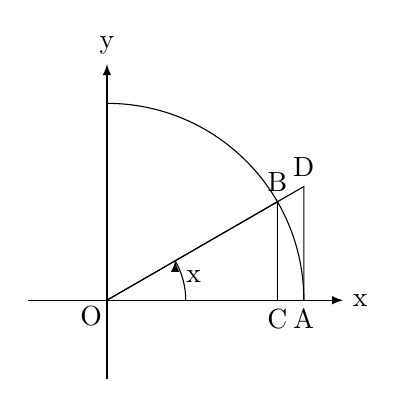
\begin{tikzpicture}[>=latex]
        \begin{scope}
            \draw[->] (-1,0)--(3,0)node[right]{x};
            \draw[->] (0,-1)--(0,3)node[above]{y};
            \draw[] (2.5,0) arc(0:90:2.5) (1,2.5);
            \draw[->] (1,0) arc(0:30:1) ({cos (pi/6 r)},{sin (pi/6 r)});
            \draw (0,0)--(30:2.5)node[above]{B}--({(2.5)*(cos (pi/6 r))},0)node[below]{C};
            \draw (0,0)--(2.5,{(2.5)*(tan (pi/6 r))})node[above]{D}--(2.5,0)node[below]{A};
            \node at (-.2,-.2) {O};
            \node at (1.1,.3) {x};
        \end{scope}
    \end{tikzpicture}
    \begin{align*}
            OB&=OA=1\\
            \vartriangle AOB&\leqslant \mbox{扇形面积}\leqslant\vartriangle AOD\\
            \frac{1}{2}\sin x&\leqslant\frac{1}{2}x\leqslant\frac{1}{2}\tan x\\
            \sin x&\leqslant x\leqslant \tan \\
            1&\geqslant\frac{\sin x}{x}\geqslant \cos x\\
            \lim\limits_{x\to 0}1&\geqslant\lim\limits_{x\to 0}\frac{\sin x}{x}\geqslant\lim\limits_{x\to 0}\cos x\\
            1&\geqslant\lim\limits_{x\to 0}\frac{\sin x}{x}\geqslant1\\
            \lim\limits_{x\to 0}\frac{\sin x}{x} &= 1
    \end{align*}
\end{center}

\textbf{\large \ref{limit_1_2}}
\begin{align*}
        \left|1-\cos x\right|=1-\cos x&=2\sin^2 \frac{x}{2}\leqslant 2\left(\frac{x}{2}\right)^2\\
        0\leqslant 1-\cos x &\leqslant \frac{x^2}{2}\\
        \lim\limits_{x\to 0}0\leqslant\lim\limits_{x\to 0}\left(1-\cos x\right)&\leqslant\lim\limits_{x\to 0}{\frac{x^2}{2}}\\
        0\leqslant\lim\limits_{x\to 0}\left(1-\cos x\right)&\leqslant 0\\
        \lim\limits_{x\to 0}\left(1-\cos x\right) &=0\\
        \lim\limits_{x\to 0}\cos x&=1
\end{align*}

\textbf{\large \ref{limit_1_3}}
\begin{align*}
        \lim\limits_{x\to 0}\frac{\tan x}{x}&=\lim\limits_{x\to 0}\frac{\sin x}{x}\frac{1}{\cos x}\\
        &=\lim\limits_{x\to 0}\frac{\sin x}{x}\lim\limits_{x\to 0}\frac{1}{\cos x}\\
        &=1
\end{align*}

\textbf{\large \ref{limit_1_4}}
\begin{align*}
        \lim\limits_{x\to 0}\frac{1-\cos x}{\frac{1}{2}x^2}&=\lim\limits_{x\to 0}\frac{2\sin^2\frac{x}{2}}{\frac{1}{2}x^2}\\
        &=\lim\limits_{x\to 0}\left(\frac{\sin \frac{x}{2}}{\frac{x}{2}}\right)^2\\
        &=1
\end{align*}

\textbf{\large \ref{limit_1_5}}
{
$$x=\sin t,\ t=\arcsin x$$
$$x\rightarrow 0,\ t\rightarrow 0$$
$$\lim\limits_{x\to 0}\frac{\arcsin x}{x}=\lim\limits_{x\to 0}\frac{t}{\sin t}=1$$
}

\textbf{\large \ref{limit_1_6}}
    {
    $$x=\tan t,\ t=\arctan x$$
    $$x\rightarrow 0,\ t\rightarrow 0$$
    $$\lim\limits_{x\to 0}\frac{\arctan x}{x}=\lim\limits_{t\to 0}\frac{t}{\tan t}=1$$
    }

\textbf{\large \ref{limit_1_7}}
\begin{align*}
        \lim\limits_{x\to 0}\frac{\ln \left(1+x\right)}{x}=\lim\limits_{x\to 0}\ln \left(1+x\right)^\frac{1}{x}=\ln e=1
\end{align*}

\textbf{\large \ref{limit_1_8}}
    $$e^x-1=t,\ x=\ln\left(t+1\right)$$
    $$x\rightarrow 0,\ t\rightarrow 0$$
    $$\lim\limits_{x\to 0}\frac{e^x-1}{x}=\lim\limits_{t\to 0}\frac{t}{\ln\left(t+1\right)}=1$$

\textbf{\large \ref{limit_1_9}}
\begin{align*}
        \lim\limits_{x\to 0}\frac{\left(1+x\right)^n-1}{nx}=\lim\limits_{x\to 0}\left(\frac{e^{n\ln \left(1+x\right)}-1}{n\ln\left(1+x\right)}\cdot\frac{\ln\left(1+x\right)}{x}\right)=1
\end{align*}

\textbf{\large \ref{limit_2_1}}
\begin{align*}
        x_n&=\left(1+\frac{1}{n}\right)^n=\sum_{m = 0}^{n} C_n^m 1^{n-m}\left(\frac{1}{n}\right)^m=\sum_{m = 0}^{n} C_n^m \left(\frac{1}{n}\right)^m\\
        &=C_n^0\left(\frac{1}{n}\right)^0+C_n^1\left(\frac{1}{n}\right)^1+ \sum_{m = 2}^{n} C_n^m \left(\frac{1}{n}\right)^m\\
        &=1+1+ \sum_{m = 2}^{n} \frac{n!}{m!\left(n-m\right)!} \left(\frac{1}{n}\right)^m\\
        &=1+1+ \sum_{m = 2}^{n} \frac{\overbrace{\left(n\right)\left(n-1\right)\cdots\left(n-m+1\right)}^{m}}{m!} \left(\frac{1}{n}\right)^m\\
        &=1+1+ \sum_{m = 2}^{n} \frac{1}{m!}\left(\frac{n}{n}\right)\left(\frac{n-1}{n}\right)\cdots\left(\frac{n-m+1}{n}\right) \\
        &=1+1+ \sum_{m = 2}^{n} \frac{1}{m!}\left(1-\frac{1}{n}\right)\left(1-\frac{2}{n}\right)\cdots\left(1-\frac{m-1}{n}\right) \\
        x_{n+1}&=1+1+ \sum_{m = 2}^{n+1} \frac{1}{m!}\left(1-\frac{1}{n+1}\right)\left(1-\frac{2}{n+1}\right)\cdots\left(1-\frac{m-1}{n+1}\right) \\
        x_n&<x_{n+1}\qquad\mbox{单调增加}\\
        x_n&<1+1+\frac{1}{2!}+\frac{1}{3!}+\cdots+\frac{1}{n!}\\
        &<1+1+\frac{1}{2^2}+\frac{1}{2^3}+\cdots+\frac{1}{n^2}=1+\frac{1-\left(\frac{1}{2}\right)^2}{1-\frac{1}{2}}\\
        &<1+\frac{1}{1-\frac{1}{2}}\\
        &<3\qquad \mbox{有界}
\end{align*}

\subsection{\centering 第\ref{chapter_derivative}章}
\textbf{\large \ref{derivative_continuity}}
\begin{align*}
        f'(x_0)&=\lim\limits_{\vartriangle x\to 0}\frac{\vartriangle y}{\vartriangle x}\qquad\mbox{因为极限存在与无穷小的关系}\\
        \frac{\vartriangle y}{\vartriangle x}&=f'(x_0)+\alpha\qquad\alpha \mbox{为}\vartriangle x\to 0\mbox{时的无穷小}\\
        \vartriangle y&=f'(x_0)\vartriangle x+\alpha\vartriangle x\\
        \lim\limits_{\vartriangle x\to 0}\vartriangle y&=\lim\limits_{\vartriangle x\to 0}\left[f'(x_0)\vartriangle x+\alpha\vartriangle x\right]=0\\
        \lim\limits_{x\to x_0}f(x)&=f(x_0)\Leftrightarrow \lim\limits_{\vartriangle x\to 0}\left[f(x_0+\vartriangle x)-f(x_0)=0\right]\Leftrightarrow\lim\limits_{\vartriangle x\to 0}\vartriangle y=0 \\
\end{align*}

\textbf{\large \ref{derivative_1}}
\begin{align*}
        (C)'&=\lim\limits_{\vartriangle x\to 0}\frac{f(x_0+\vartriangle x)-f(x_0)}{\vartriangle x}\\
        &=\lim\limits_{\vartriangle x\to 0} \frac{C-C}{\vartriangle x}\\
        &=0
\end{align*}

\textbf{\large \ref{derivative_2}}
\begin{align*}
        \left(x^a\right)'&=\lim\limits_{x\to x_0}\frac{f(x)-f(x_0)}{x-x_0}\\
        &=\frac{x^a-x_0^a}{x-x_0}\\
        &=\frac{(x-x_0)\left(x^{a-1}+x^{a-2}x_0+\cdots+xx_0^{a-2}+x_0^{a-1}\right)}{x-x_0}\\
        &=ax_0^{a-1}
\end{align*}

\textbf{\large \ref{derivative_3}}
\begin{align*}
        \left(a^x\right)'&=\lim\limits_{\vartriangle x\to 0}\frac{a^{x+\vartriangle x}-a^x}{\vartriangle x}\\
        &=a^x\lim\limits_{\vartriangle x\to 0}\frac{a^{\vartriangle x}-1}{\vartriangle x}\\
        &=a^x\lim\limits_{\vartriangle x\to 0}\frac{e^{\vartriangle x \ln a}-1}{\vartriangle x}\\
        &=a^x\ln a
\end{align*}

\textbf{\large \ref{derivative_4}}
\begin{align*}
        \left(e^x\right)'=e^x\ln e=e^x
\end{align*}

\textbf{\large \ref{derivative_5}}
\begin{align*}
        \left(\log_a^x\right)'&=\lim\limits_{\vartriangle x\to 0}\frac{\log_a^{x+\vartriangle x}-\log_a^x}{\vartriangle x}\\
        &=\lim\limits_{\vartriangle x\to 0}\frac{\log_a^{1+\frac{\vartriangle x}{x}}}{\vartriangle x}\\
        &=\lim\limits_{\vartriangle x\to 0}\frac{\ln{1+\frac{\vartriangle x}{x}}}{\ln a\vartriangle x}\\
        &=\frac{1}{\ln a}\lim\limits_{\vartriangle x\to 0}\frac{\frac{\vartriangle x}{x}}{\vartriangle x}\\
        &=\frac{1}{x\ln a}
\end{align*}

\textbf{\large \ref{derivative_6}}
\begin{align*}
        \left(\ln^x\right)'&=\frac{1}{x\ln e}\\
        &=\frac{1}{x}
\end{align*}

\textbf{\large \ref{derivative_sin}}
\begin{align*}
        (\sin x)'&=\lim\limits_{\vartriangle x\to 0}\frac{\sin (x_0 +\vartriangle x)-\sin x_0}{\vartriangle x}\\
        &=\lim\limits_{\vartriangle x\to 0}\frac{2\cos(x_0+\frac{\vartriangle x}{2})\sin \frac{\vartriangle x}{2}}{\vartriangle x}\\
        &=\lim\limits_{\vartriangle x\to 0}\cos(x_0+\frac{\vartriangle x}{2})\frac{\sin\frac{\vartriangle x}{2}}{\frac{\vartriangle x}{2}}\\
        &=cos x_0
\end{align*}

\textbf{\large \ref{derivative_arcsin}}
\begin{align*}
        (\arcsin x)'=\frac{1}{\frac{dx}{\mathrm{d}{y}}}&=\frac{1}{\frac{d\sin y}{\mathrm{d}{y}}}\\
        &=\frac{1}{\cos y}\\
        &=\frac{1}{\sqrt{1-\sin^2 y}}\\
        &=\frac{1}{\sqrt{1-x^2}}
\end{align*}

\textbf{\large \ref{derivative_csc}}
\begin{align*}
        (\csc x)'=(\frac{1}{\sin x})‘&=\frac{(1)'\cdot sin x-(\sin x)'\cdot 1}{\sin^2x}\\
        &=\frac{-\cos x}{\sin^2x}\\
        &=-\csc x\cdot\cot x
\end{align*}

\textbf{\large \ref{derivative_cos}}
\begin{align*}
        (\cos x)'&=\lim\limits_{\vartriangle x\to 0}\frac{\cos(x_0+\vartriangle x)-cos(x_0)}{\vartriangle x}\\
        &=\lim\limits_{\vartriangle x\to 0}\frac{-2\sin \left(x_0+\frac{\vartriangle x}{2}\right)\sin\frac{\vartriangle x}{2}}{\vartriangle x}\\
        &=\lim\limits_{\vartriangle x\to 0}-\sin \left(x_0+\frac{\vartriangle x}{2}\right)\frac{\sin\frac{\vartriangle x}{2}}{\frac{\vartriangle x}{2}}\\
        &=-\sin x
\end{align*}

\textbf{\large \ref{derivative_arccos}}
\begin{align*}
        (\arccos x)'=\frac{1}{\frac{dx}{\mathrm{d}{y}}}&=\frac{1}{\frac{d\cos y}{\mathrm{d}{y}}}\\
        &=\frac{1}{-\sin y}\\
        &=-\frac{1}{\sqrt{1-\cos^2 y}}\\
        &=-\frac{1}{\sqrt{1-x^2}}
\end{align*}

\textbf{\large \ref{derivative_sec}}
\begin{align*}
        (\sec x)'=\left(\frac{1}{\cos x}\right)'&=\frac{(1)'\cdot\cos x-(\cos x)'\cdot 1}{\cos^2x}\\
        &=\frac{\sin x}{\cos^2x}\\
        &=\sec x\cdot\tan x
\end{align*}

\textbf{\large \ref{derivative_tan}}
\begin{align*}
        (\tan x)'=\left(\frac{\sin x}{\cos x}\right)'&=\frac{(\sin x)'\cos x-(\cos x)'\sin x}{\cos^2x}\\
        &=\frac{\cos^2 x+\sin^2 x}{\cos^2x}\\
        &=\sec^2 x
\end{align*}

\textbf{\large \ref{derivative_arctan}}
\begin{align*}
        (\arctan x)'=\frac{1}{\frac{dx}{\mathrm{d}{y}}}&=\frac{1}{\frac{d\tan y}{\mathrm{d}{y}}}\\
        &=\frac{1}{\sec y}\\
        &=\frac{1}{1+\tan^2 y}\\
        &=\frac{1}{1+x^2}
\end{align*}

\textbf{\large \ref{derivative_cot}}
\begin{align*}
        (\cot x)'=\left(\frac{\cos x}{\sin x}\right)'&=\frac{(\cos x)'\sin x-(\sin x)'\cos x}{\sin^2x}\\
        &=-\frac{\sin^2 x+\cos^2 x}{\cos^2x}\\
        &=-\csc^2 x
\end{align*}

\textbf{\large \ref{derivative_arccot}}
\begin{align*}
        (\operatorname{arccot}{x})'=\frac{1}{\frac{dx}{\mathrm{d}{y}}}&=\frac{1}{\frac{d\cot y}{\mathrm{d}{y}}}\\
        &=\frac{1}{-\csc^2 y}\\
        &=-\frac{1}{1+\cot^2 y}\\
        &=-\frac{1}{1+x^2}
\end{align*}

\textbf{\large \ref{derivative_sinh}}
\begin{align*}
        (\sinh x)'&=\left(\frac{e^x-e^{-x}}{2}\right)'\\
                                    &=\frac{e^x+e^{-x}}{2}\\
                                    &=\cosh x
\end{align*}
\textbf{\large \ref{derivative_cosh}}
\begin{align*}
        (\cosh x)'&=\left(\frac{e^x+e^{-x}}{2}\right)'\\
                                    &=\frac{e^x-e^{-x}}{2}\\
                                    &=\sinh x
\end{align*}

\textbf{\large \ref{derivative_tanh}}
\begin{align*}
        (\tanh x)'&=\left(\frac{e^x-e^{-x}}{e^x+e^{-x}}\right)'\\
                                    &=\frac{\frac{d(e^x-e^{-x})}{\mathrm{d}{x}}(e^x+e^{-x})-\frac{d(e^x+e^{-x})}{\mathrm{d}{x}}(e^x-e^{-x})}{\left(e^x+e^{-x}\right)^2}\\
                                    &=\frac{\left(e^x+e^{-x}\right)^2-\left(e^x-e^{-x}\right)^2}{\left(e^x+e^{-x}\right)^2}\\
                                    &=\frac{2^2}{\left(e^x+e^{-x}\right)^2}\\
                                    &=\frac{1}{\cosh^2 x}
\end{align*}

\textbf{\large \ref{derivative_arcsinh}}
\begin{align*}
        (\operatorname{arcsinh}{x})' &=\left[\ln(x+\sqrt{x^2+1})\right]'\\
                                    &=\frac{d \ln(x+\sqrt{x^2+1})}{\mathrm{d}{\left(x+\sqrt{x^2+1}\right)}}\cdot\frac{d \left(x+\sqrt{x^2+1}\right)}{\mathrm{d}{x}}\\
                                    &=\frac{1}{x+\sqrt{x^2+1}}\cdot\left(\frac{dx}{dx}+\frac{d \left(\sqrt{x^2+1}\right)}{d\left(x^2+1\right)}\cdot\frac{d(x^2+1)}{dx}\right)\\
                                    &=\frac{1}{x+\sqrt{x^2+1}}\cdot\left(1+\frac{1}{2\sqrt{x^2+1}}\cdot 2x\right)\\                                    
                                    &=\frac{1}{x+\sqrt{x^2+1}}\cdot\frac{x+\sqrt{x^2+1}}{\sqrt{x^2+1}}\\
                                    &=\frac{1}{\sqrt{x^2+1}}
\end{align*}

\textbf{\large \ref{derivative_arccosh}}
\begin{align*}
        (\operatorname{arccosh}{x})' &=\left[\ln(x+\sqrt{x^2-1})\right]'\\
                                    &=\frac{d \ln(x+\sqrt{x^2-1})}{\mathrm{d}{\left(x+\sqrt{x^2-1}\right)}}\cdot\frac{d \left(x+\sqrt{x^2-1}\right)}{\mathrm{d}{x}}\\
                                    &=\frac{1}{x+\sqrt{x^2-1}}\cdot\left(\frac{dx}{dx}+\frac{d \left(\sqrt{x^2-1}\right)}{d\left(x^2-1\right)}\cdot\frac{d(x^2-1)}{dx}\right)\\
                                    &=\frac{1}{x+\sqrt{x^2-1}}\cdot\left(1+\frac{1}{2\sqrt{x^2-1}}\cdot 2x\right)\\                                    
                                    &=\frac{1}{x+\sqrt{x^2-1}}\cdot\frac{x+\sqrt{x^2-1}}{\sqrt{x^2-1}}\\
                                    &=\frac{1}{\sqrt{x^2-1}}
\end{align*}

\textbf{\large \ref{derivative_arctanh}}
\begin{align*}
        (\operatorname{arctanh}{x})' &=\left[\frac{1}{2}\ln(\frac{1+x}{1-x})\right]'\\
        &=\frac{1}{2}\cdot\frac{d\left[\ln(\frac{1+x}{1-x})\right]}{\mathrm{d}{\left(\frac{1+x}{1-x}\right)}}\cdot\frac{d\left(\frac{1+x}{1-x}\right)}{\mathrm{d}{x}}\\
        &=\frac{1}{2}\cdot\frac{1}{\left(\frac{1+x}{1-x}\right)}\cdot\frac{\frac{d(1+x)}{\mathrm{d}{x}}(1-x)-\frac{d(1-x)}{\mathrm{d}{x}}(1+x)}{(1-x)^2}\\
        &=\frac{1}{2}\cdot\frac{1-x}{1+x}\cdot\frac{(1-x)+(1+x)}{(1-x)^2}\\
        &=\frac{1}{(1+x)(1-x)}\\
        &=\frac{1}{1-x^2}
\end{align*}

\textbf{\large \ref{limit_operation_1}}
\begin{align*}
        \left[Cu(x)\right]'&=\lim\limits_{\vartriangle x\to 0}\frac{Cu(x+\vartriangle x)-Cu(x)}{\vartriangle x}\\
        &=C\lim\limits_{\vartriangle x\to 0}\frac{u(x+\vartriangle x)-u(x)}{\vartriangle x}\\
        &=Cu'(x)
\end{align*}
\textbf{\large \ref{limit_operation_2}}
\begin{align*}
            (u(x)\pm v(x))'&=\lim\limits_{\vartriangle x\to 0}\frac{u(x+\vartriangle x)-u(x)\pm v(x+\vartriangle x)-v(x)}{\vartriangle x}\\
        &=\lim\limits_{\vartriangle x\to 0}\frac{u(x+\vartriangle x)-u(x)}{\vartriangle x}\pm\lim\limits_{\vartriangle x\to 0}\frac{v(x+\vartriangle x)-v(x)}{\vartriangle x}\\
        &=u'(x)\pm v'(x)
\end{align*}
\textbf{\large \ref{limit_operation_3}}
\begin{align*}
        \left[u(x)\cdot v(x)\right]'&=\lim\limits_{\vartriangle x\to 0}\frac{u(x+\vartriangle x)v(x+\vartriangle x)-u(x)v(x)-u(x)v(x+\vartriangle x)+u(x)v(x+\vartriangle x)}{\vartriangle x}\\
            &=\lim\limits_{\vartriangle x\to 0}\frac{\left[u(x+\vartriangle x)-u(x)\right]v(x+\vartriangle x)+u(x)\left[v(x+\vartriangle x)-v(x)\right]}{\vartriangle x}\\
            &=u'(x)\lim\limits_{\vartriangle x\to 0}v(x+\vartriangle x)+u(x)v'(x)\\
            &=u'(x)v(x)+v'(x)u(x)
\end{align*}
\textbf{\large \ref{derivative_of_inverse_function}}
\begin{align*}
        \left[f^{-1}(y)\right]'|_{y=y_0}&=\lim\limits_{y\to y_o}\frac{f^{-1}(y)-f^{-1}(y_0)}{y-y_0}\\
        &=\lim\limits_{y\to y_o}\frac{x-x_0}{y-y_0}\\
        &=\lim\limits_{x\to x_o}\frac{x-x_0}{f(x)-f(x_0)}\\
        &=\lim\limits_{x\to x_o}\frac{1}{\frac{f(x)-f(x_0)}{x-x_0}}\\
        &=\frac{1}{f'(x)}
\end{align*}

\textbf{\large \ref{derivative_of_composite_functions}}
$$        \mbox{定义函数}\quad A(u)=\begin{cases}
    \frac{f(u)-f(u_0)}{u-u_0}. &u\neq u_0\\
    f'(u_0),&u= u_0
\end{cases}$$
$$A(u)\mbox{在}u_o\mbox{处连续,既有,}\ \lim\limits_{u\to u_o}A(u)=A(u_0)=f'(u_0)$$
\begin{align*}
        \mbox{由恒等式}f(u)-f(u_0)&=A(u)(u-u_0)\mbox{我们有}\\
        \frac{F(x)-F(x_0)}{x-x_0}&=\frac{f\left[g(x)\right]-f\left[g(x_0)\right]}{x-x_0}\\
        &=A\left[g(x)\right]\frac{g(x)-g(x_0)}{x-x_0}\\
        \lim\limits_{x\to x_0}\frac{F(x)-F(x_0)}{x-x_0}&=\lim\limits_{x\to x_0}A\left[g(x)\right]\frac{g(x)-g(x_0)}{x-x_0}\\
        F'(x_0)&=f'(g(x_0))g'(x_0)
\end{align*}

\subsection{\centering 第\ref{chapter_differential}章}
\textbf{\large \ref{differential_to_derivative}}
\begin{align*}
            \vartriangle y&=A\vartriangle x+\circ(\vartriangle x)\\
            \frac{\vartriangle y}{\vartriangle x}&=A+\frac{\circ(\vartriangle x)}{\vartriangle x}\\
            \lim\limits_{\vartriangle x\to 0}\frac{\vartriangle y}{\vartriangle x}&=\lim\limits_{\vartriangle x\to 0}\left[A+\frac{\circ(\vartriangle x)}{\vartriangle x}\right]\\
            f'(x_0)&=A+0\\
            f'(x_0)&=A
\end{align*}
\textbf{\large \ref{derivative_to_differential}}
\begin{center}
            $\mbox{设}f(x)\mbox{在}x_0\mbox{点可导},f'(x_0)=\lim\limits_{\vartriangle x \to 0}\frac{\vartriangle y}{\vartriangle x}\mbox{存在}$\\
            $\left(\mbox{极限与无穷小的关系:}\lim f(x)=A\Leftrightarrow f(x)=A+\alpha\right)$\\
            $\frac{\vartriangle y}{\vartriangle x}=f'(x_0)+\alpha$\\
            $\vartriangle y=f'(x_0)\vartriangle x+\alpha \vartriangle x$\\
            $\mbox{其中}\alpha \mbox{为}\vartriangle x\to 0\mbox{时的无穷小。}$\\
            $\lim\limits_{\vartriangle x\to 0}\frac{\alpha \vartriangle x}{\vartriangle x}=\lim\limits_{\vartheta x\to 0}\alpha = 0$\\
            $\alpha \vartriangle x=\circ(\vartriangle x)$\\
            $\vartriangle y=f'(x_0)\vartriangle x+\circ(\vartriangle x)$
\end{center}

\textbf{\large \ref{differential_operation_rule_1}}
\begin{align*}
        d(u\pm v)&=(u\pm v)'dx\\
                &=(u)'dx \pm (v')dx\\
                &=du\pm dv
\end{align*}

\textbf{\large \ref{differential_operation_rule_2}}
\begin{align*}
        d(u\cdot v)&=(u\cdot v)'dx\\
                &=(u)'vdx - (v')udx\\
                &=vdu - udv
\end{align*}

\textbf{\large \ref{differential_operation_rule_3}}
\begin{align*}
        d\left(\frac{u}{v}\right)&=\left(\frac{u}{v}\right)'dx\\
                &=\frac{(u)'v - (v')u}{v^2}dx\\
                &=\frac{vdu - udv}{v^2}
\end{align*}

\textbf{\large \ref{Fermat_Lemma}}
\begin{center}
    $\lim\limits_{\vartriangle x\to 0}\frac{f(x_0+\vartriangle x)}{\vartriangle x}=f'(x_0)$\\
    $f(x_0+\vartriangle x)-f(x_0)\leqslant 0$\\
    $\begin{cases}
        \vartriangle x>0\begin{cases}
            \frac{f(x_0+\vartriangle x)-f(x_0)}{\vartriangle x}\leqslant 0\Rightarrow f'(x_0^+) =\lim\limits_{\vartriangle x \to 0}\frac{f(x_0+\vartriangle x)-f(x_0)}{\vartriangle x}\leqslant 0
        \end{cases}\\
        \vartriangle x<0\begin{cases}
            \frac{f(x_0+\vartriangle x)-f(x_0)}{\vartriangle x}\geqslant 0\Rightarrow f'(x_0^-) =\lim\limits_{\vartriangle x \to 0}\frac{f(x_0+\vartriangle x)-f(x_0)}{\vartriangle x}\geqslant 0
        \end{cases}
    \end{cases}$\\
    $f'(x_0)=f'(x_0^+)=f'(x_0^-)\Rightarrow f'(x_0)= 0$
\end{center}

\textbf{\large \ref{Rolle's theorem}}
\begin{center}
    $M=\max\{f(x)|x\in[a,b]\},m=\min\{f(x)|x\in[a,b]\}$
    $\begin{cases}
        M=m\Rightarrow M=m=f(a)=f(b),\mbox{此时}f(x)\mbox{为常数},\forall \xi \in(a,b),f'(\xi)=0\\
        M>m \begin{cases}
            f(a)>m \Rightarrow \exists \xi \in(a,b),f(\xi)=m,\mbox{根据费马引理},f'(\xi)=0\\
            f(a)<M5 \Rightarrow \exists \xi \in(a,b),f(\xi)=M,\mbox{根据费马引理},f'(\xi)=0\\
        \end{cases}
    \end{cases}$
\end{center}
\textbf{\large \ref{Lagrange's theorem}}
\begin{align*}
        \varphi(x)&=f(x)-\frac{f(b)-f(a)}{b-a}x\\
        \varphi(a)&=f(a)-\frac{f(b)-f(a)}{b-a}a=\frac{bf(a)-af(b)}{b-a}\\
        \varphi(b)&=f(b)-\frac{f(b)-f(a)}{b-a}b=\frac{bf(a)-af(b)}{b-a}\\
        \varphi(a)&=\varphi(b),\exists \xi\in(a,b),\varphi'(\xi)=0\\
        f'(\xi)&=\frac{f(b)-f(a)}{b-a}\\
        f'(\xi)(b-a)&7=f(b)-f(a)
\end{align*}

\textbf{\large \ref{cauchy_theorem}}
\begin{align*}
        \varphi(x)&=f(x)-\frac{f(b)-f(a)}{F(b)-F(a)}\left[F(x)-F(a)\right] \\
        \varphi(a)&=\varphi(b)=f(a)\\
        \varphi'(\xi)&=0\\
        f'(\xi)&=\frac{f(b)-f(a)}{F(b)-F(a)}F'(\xi)\\
        \frac{f'(\xi)}{F'(\xi)}&=\frac{f(b)-f(a)}{F(b)-F(a)}
\end{align*}

\textbf{\large \ref{l'hospital rule}}
    \begin{center}
        $f(x),F(x)\mbox{的去心邻域可导,}\lim\limits_{x\to x_0}\frac{f(x)}{F(x)}\mbox{与}f(x_0),F(x_0)\mbox{无关。规定}f(x_0)=0,F(x_0)=0$\\
$\mbox{此时}\lim\limits_{x\to x_0}f(x)=0=f(x_0)\quad\lim\limits_{x\to x_0}F(x)=0=F(x_0)\quad\mbox{此时在$x_0$点处也连续}$\\
    \end{center}
    \begin{align*}
    \frac{f(x)}{F(x)}&=\frac{f(x)-f(x_0)}{F(x)-F(x_0)}=\frac{f'(\xi)}{F'(\xi)}\\
    \lim\limits_{x\to x_0}\frac{f(x)}{F(x)}&=\lim\limits_{x\to x_0}\frac{f'(\xi)}{F'(\xi)}\\
    x\rightarrow x_0,&\mbox{时}\xi\rightarrow x_0\qquad \mbox{符号$\xi$换成x}\\
    \lim\limits_{x\to x_0}\frac{f(x)}{F(x)}&=\lim\limits_{\xi\to x_0}\frac{f'(\xi)}{F'(\xi)}=\lim\limits_{x\to x_0}\frac{f'(x)}{F'(x)}
    \end{align*}

\textbf{\large \ref{lagrange_remainder}}
\begin{align*}
    \frac{R_n(x)}{(x-x_0)^{n+1}}&=\frac{R_n(x)-R_n(x_0)}{(x-x_0)^{n+1}-(x_0-x_0)^{n+1}}=\frac{R_n'(\xi_1)}{(n+1)(\xi_1-x_0)^n}\\
    \frac{1}{n+1}\cdot\frac{R_n'(\xi_1)}{(\xi_2-x_0)^n}&=\frac{1}{n+1}\cdot\frac{R_n'(\xi_1)-R_n'(x_0)}{(\xi_1-x_0)^{n}-(x_0-x_0)^{n}}=\frac{1}{n+1}\cdot\frac{R_n''(\xi_2)}{(n)(\xi_2-x_0)^{n-1}}\\
    &\vdots\\
    \frac{R_n^{(n)}(\xi_n)}{(n+1)!(\xi_n-x_0)}&=\frac{R_n^{(n)}(\xi_n)-R_n^{(n)}(x_0)}{(n+1)!(\xi_n-x_0)-0}=\frac{R_n^{(n+1)}(\xi)}{(n+1)!}\\
    \frac{R_n^{(n+1)}(\xi)}{(n+1)!}&=\frac{f^{(n+1)}(\xi)-P_n^{(n+1)}(\xi)}{(n+1)!}=\frac{f^{(n+1)}(\xi)}{(n+1)!}\\
    R_n(x)&=\frac{f^{(n+1)}(\xi)}{(n+1)!}(x-x_0)^{n+1}
\end{align*}
\centerline{$\xi_1\in(x,x_0),\xi_2\in(\xi_1,x_0),\xi_n\in(\xi_{n-1},x_0),\xi\in(\xi_n,x_0)$}

\textbf{\large \ref{Piano_remainder}}
\begin{align*}
      \lim\limits_{x\to x_0}\frac{R_n(x)}{(x-x_0)^n}&=\lim\limits_{x\to x_0}\frac{R_n'(x)}{n(x-x_0)^{n-1}}\\
      &=\lim\limits_{x\to x_0}\frac{R_n''(x)}{n(n-1)(x-x_0)^{n-2}}\\
      &=\lim\limits_{x\to x_0}\frac{R_n^{(n)}(x)}{n!}\\
      &=\frac{1}{n}\cdot 0\\
      &=0
\end{align*}
\subsection{\centering 第\ref{differential_equations}章}
\textbf{\large \ref{First_order_linear_differential_equation_1}}
\begin{align*}
	\frac{dy}{dx}+P(x)y&=0\\
	\frac{dy}{y}&=-P(x)\ dx\\
	\int \frac{dy}{y}&=\int -P(x)\ dx\\
	\ln\left|y\right|&=-\int P(x)\ dx+C_2\\
	\left|y\right|&=C_1e^{-\int P(x)\ dx}\\
	y&=Ce^{-\int P(x)\ dx}
\end{align*}
\textbf{\large \ref{First_order_linear_differential_equation_2}}\\
\centerline{\textbf{常数变异法:假设一个解,包含关于$x$的未知函数$u(x)$}}
\begin{align*}
	y&=Ce^{-\int P(x)\ dx}\\
	y&=u(x)e^{-\int P(x)\ dx}\\
	\frac{dy}{dx}&=u'(x)e^{-\int P(x)\ dx}+u(x)e^{-\int P(x)\ dx}\cdot\left[-P(x)\right]\\
	\frac{dy}{dx}&=u'(x)e^{-\int P(x)\ dx}-P(x)u(x)e^{-\int P(x)\ dx}
\end{align*}
\centerline{\textbf{$u(x)$的表达式带入原方程,求出$u(x)$与$Q(x)$的关系}}
\begin{align*}
	\frac{dy}{dx}+P(x)y&=Q(x)\\
	u'(x)e^{-\int P(x)\ dx}-P(x)u(x)e^{-\int P(x)\ dx}+P(x)u(x)e^{-\int P(x)\ dx}&=Q(x)\\
	u'(x)e^{-\int P(x)\ dx}&=Q(x)\\
	u'(x)&=Q(x)e^{\int P(x)\ dx}\\
	u(x)&=\int Q(x)e^{\int P(x)\ dx}\ dx+C
\end{align*}
\centerline{\textbf{求出$u(x)$与$Q(x)$的关系,在带回假设的解}}
\begin{align*}
	y&=u(x)e^{-\int P(x)\ dx}\\
	y&=e^{-\int P(x)\ dx}\left[\int Q(x)e^{\int P(x)\ dx}\ dx+C\right]
\end{align*}
\textbf{\large \ref{second_order_linear_differential_equation_1}}\\
\begin{minipage}{.5\textwidth}
	\begin{align*}
y_1''(x)+P_1(x)y_1'+P_2(x)y_1\equiv 0\\
y_2''(x)+P_1(x)y_2'+P_2(x)y_2\equiv 0
	\end{align*}
\end{minipage}
\hfill
\vline
\begin{minipage}{.5\textwidth}
	\begin{align*}
	y&=C_1y_1+C_2y_2\\
	y'&=C_1y_1'+C_2y_2'\\
	y''&=C_1y_1''+C_2y_2''
	\end{align*}
\end{minipage}
\begin{align*}
	&y''+P_1(x)y'+P_2(x)y\\
	=&C_1y_1''+C_2y_2''+P_1(x)\left(C_1y_1'+C_2y_2'\right)+P_2(x)\left(C_1y_1+C_2y_2\right)\\
	=&C_1\left[y_1''(x)+P_1(x)y_1'+P_2(x)y_1\right]+C_2\left[y_2''(x)+P_1(x)y_2'+P_2(x)y_2\right]\\
	\equiv &0
\end{align*}
\textbf{\large \ref{Second_order_homogeneous_differential_equation_with_constant_coefficients}}\\
\noindent\rule[\fill]{\textwidth}{0.4pt}
\begin{minipage}{.2\textwidth}
	\centerline{\textbf{特征方程}}
\end{minipage}
\hfill
\vline
\begin{minipage}{.8\textwidth}
	\begin{align*}
		y''+py'+qy=0\\
		r^2e^{rx}+pre^{rx}+qe^{rx}=0\\
		e^{rx}(r^2+pr+q)=0\\
		r^2+pr+q=0
	\end{align*}
\end{minipage}
\noindent\rule[\fill]{\textwidth}{0.4pt}
\begin{minipage}{.2\textwidth}
	\begin{align*}
		p^2-4q>0
	\end{align*}
\end{minipage}
\hfill
\vline
\begin{minipage}{.8\textwidth}
	\begin{align*}
		\mbox{两个不同实根解:}r_1,r_2\\
		\frac{e^{r_1x}}{e^{r_2x}}=e^{(r_1-r_2)x}\not\equiv\mbox{常数}\qquad\mbox{线性无关}\\
		y=C_1y_1+C_2y_2=C_1e^{r_1x}+C_2e^{r_2x}
	\end{align*}
\end{minipage}
\noindent\rule[\fill]{\textwidth}{0.4pt}
\begin{minipage}{.2\textwidth}
	\begin{align*}
		p^2-4q=0
	\end{align*}
\end{minipage}
\hfill
\vline
\begin{minipage}{.8\textwidth}
	$$\mbox{两个相同解:}r_1=r_2=-\frac{p}{2}\ \mbox{设}y_2=u(x)e^{r_1x}\mbox{是另一个解}$$
	\begin{align*}
		y_2'&=u'e^{r_1x}+r_1ue^{r_1x}=(u'+r_1u)e^{r_1x}\\
		y_2''&=(u''+r_1)e^(r_1x)+(u'+r_1u)e^{r_1x}r_1=(u''+2r_1u'+r_1^2u)e^{r_1x}
	\end{align*}
	\begin{align*}
		y''+py'+qy=0\\
		(u''+2r_1u'+r_1^2u)e^{r_1x}+p(u'+r_1u)e^{r_1x}+que^{r_1x}=0\\
		e^{r_1x}\left[u''+(2r_1+p)+(r_1^2+pr_1+q)u\right]=0\\
		u''=0
	\end{align*}
	$$u=C_1x+C_2 \quad\mbox{取:}u(x)=x\quad\frac{e^{r_1x}}{xe^{r_1x}}=xe^{(r_1-r_2)x}\not\equiv\mbox{常数}$$
	$$y=C_1y_1+C_2y_2=C_1e^{r_1x}+C_2xe^{r_1x}$$
\end{minipage}
\noindent\rule[\fill]{\textwidth}{0.4pt}
\begin{minipage}{.2\textwidth}
	\begin{align*}
		p^2-4q<0
	\end{align*}
\end{minipage}
\hfill
\vline
\begin{minipage}{.8\textwidth}
	$$\mbox{两个共轭复根解:}r_{1,2}=\alpha\pm i\beta$$
	$$y_1=e^{(\alpha+i\beta)x}=e^{\alpha x}(\cos\beta x+i\sin\beta x)$$
	$$y_2=e^{(\alpha=i\beta)x}=e^{\alpha x}(\cos\beta x-i\sin\beta x)$$
	$$\overline{y_1}=\frac{1}{2}(y_1+y_2)=e^{\alpha x}\cos\beta x$$
	$$\overline{y_2}=\frac{1}{2i}(y_1-y_2)=e^{\alpha x}\sin\beta x$$
	$$\frac{\overline{y_1}}{\overline{y_2}}=\cot\beta x\not\equiv\mbox{常数}$$
	$$y=C_1\overline{y_1}+C_2\overline{y_2}=e^{\alpha x}(C_1\cos\beta x+C_2\sin\beta x)$$
\end{minipage}
\noindent\rule[\fill]{\textwidth}{0.4pt}
\subsection{\centering 第\ref{chapter_Indefinite_integral}章}
\textbf{\large \ref{Indefinite_integral_operation_1}}
\begin{align*}
    \left[\int f(x)\ dx \pm \int g(x)\ dx\right]'&=\left[\int f(x) \ dx\right]'\pm \left[\int g(x) \ dx\right]'\\
    &=f(x) \pm g(x)
\end{align*}

\textbf{\large \ref{Indefinite_integral_operation_2}}
\begin{align*}
    \left[k\int f(x)\ dx\right]'&=k\left[\int f(x)\ dx\right]'\\
    &=kf(x)
\end{align*}

\textbf{\large \ref{Indefinite_integral_operation_3}}
\begin{align*}
    \left\{F\left[\varphi(x)\right]\right\}'&=F'\left[\varphi (x)\right]\varphi'(x)\\
    &=f\left[\varphi(x)\right]\varphi'(x)
\end{align*}

\textbf{\large \ref{Indefinite_integral_operation_4}}
\begin{align*}
    x&=\varphi(t)\\
    dx&=d\varphi(t)\\
    dx&=\varphi'(t)dt\\
    \int f(x)\ dx&=\int f\left[\varphi(t)\right]\varphi'(t) \ dt
\end{align*}

\textbf{\large \ref{Indefinite_integral_operation_5}}
\begin{align*}
    \int f(x)\ dx&=\int f(x)\cdot(x+C)'\ dx\\
    &=\int f(x)\ d(x+C)
\end{align*}

\textbf{\large \ref{integral_0_1}}
\begin{align*}
        \int k\ dx=\int (kx)'\ dx=kx+C
\end{align*}

\textbf{\large \ref{integral_0_2}}
\begin{align*}
        \int x^a\ dx=\int \left(\frac{1}{a+1}x^{a+1}\right)'\ dx=\frac{x^{a+1}}{a+1}+C
\end{align*}

\textbf{\large \ref{integral_0_3}}
\begin{align*}
        \int a^x\ dx=\int \left(\frac{1}{\ln a}a^x\right)'\ dx=\frac{a^x}{\ln a}+C
\end{align*}

\textbf{\large \ref{integral_0_4}}
\begin{align*}
        \int e^x\ dx=\int (e^x)'\ dx=e^x+C
\end{align*}

\textbf{\large \ref{integral_0_5}}
\begin{align*}
        \int \frac{1}{x}\ dx=\begin{cases}
                (x>0)\qquad\int (\ln x)'\ dx=\ln x+C=\ln \left|x\right|+C\\
                (x<0)\qquad\int \left[\ln (-x)\right]'\ dx=\ln(-x)+C=\ln \left|x\right|+C
        \end{cases}
\end{align*}

\textbf{\large \ref{integral_0_6}}
\begin{align*}
        \int \ln x\ dx&= \ln x\cdot x-\int x\ d\ln x\\
        &= x\ln x-\int x\cdot \frac{1}{x}\ dx\\
        &=x\ln x- x+C
\end{align*}

\textbf{\large \ref{integral_sin}}
\begin{align*}
        \int \sin x\ dx=\int (-\cos x)'\ dx=-\cos x +C
\end{align*}

\textbf{\large \ref{integral_cos}}
\begin{align*}
        \int \cos x\ dx=\int (\sin x)'\ dx=\sin x+C
\end{align*}

\textbf{\large \ref{integral_sec_tan}}
\begin{align*}
        \int \sec x\tan x\ dx= \int (\sec x)'\ dx= \sec x
\end{align*}

\textbf{\large \ref{integral_csc_cot}}
\begin{align*}
        \int \csc x\cot x\ dx= -\int (\csc x)'\ dx= -\csc x
\end{align*}

\textbf{\large \ref{integral_sec_sec}}
\begin{align*}
        \int \sec^2 x\ dx=\int (\tan x)'\ dx=\tan x
\end{align*}

\textbf{\large \ref{integral_csc_csc}}
\begin{align*}
        \int \csc^2 x\ dx=-\int (\cot x)'\ dx=-\cot x
\end{align*}

\textbf{\large \ref{integral_tan}}
\begin{align*}
        \int \tan x\ dx&=\int \frac{\sin x}{\cos x}\ dx\\
           &=-\int \frac{(\cos x)'}{\cos x}\ dx\\
           &=-\int \frac{1}{\cos x}\ d(\cos x)\\
           &=-\ln\left|\cos x\right|+C
\end{align*}

\textbf{\large \ref{integral_csc}}
\begin{align*}
    \int \csc x\ dx&=\int \frac{1}{\sin x}\ dx\\
    &=\int \frac{1}{2\sin\frac{x}{2}\cos\frac{x}{2}}\ dx\\
    &=\int \frac{1}{\tan \frac{x}{2}}\cdot \frac{1}{\cos^2\frac{x}{2}}\ d\frac{x}{2}\\
    &=\int \frac{1}{\tan \frac{x}{2}}\cdot \sec^2\frac{x}{2}\ d\frac{x}{2}\\
    &=\int \frac{1}{\tan \frac{x}{2}}\ d \tan \frac{x}{2}\\
    &=\begin{cases}
        \ln \left|\tan \frac{x}{2}\right|+C\\
        \ln \left|\csc x - \cot x\right|+C
    \end{cases}
\end{align*}

\textbf{\large \ref{integral_sec}}
\begin{align*}
        \int \sec x\ dx&=\int \frac{1}{\cos x}\ dx\\
        &=\int \frac{\cos x}{\cos^2x}\ dx\\
        &=\int \frac{1}{\cos^2x}\ d\sin x\\
        &=\int \frac{1}{1-\sin^2 x}\ d\sin x\\
        &=\frac{1}{2}\ln\left|\frac{1+\sin x}{1-\sin x}\right|+C\\
        &=\frac{1}{2}\left|\frac{1+\sin x}{\cos x}\right|^2+C\\
        &=\ln\left|\sec x+\tan x\right|+C
\end{align*}

\textbf{\large \ref{integral_arccos}}
\begin{align*}
        \int \arccos x\ dx&= x\arccos x-\int x \cdot-\frac{1}{\sqrt{1-x^2}}\ dx\\
        &= x\arccos x-\frac{1}{2}\int  \frac{1}{\sqrt{1-x^2}}\ d(1-x^2)\\
        &= x\arccos x-\frac{1}{2}\cdot\frac{1}{-\frac{1}{2}+1} (1-x^2)^{-\frac{1}{2}+1}+C \\
        &= x\arccos x-\sqrt{1-x^2} +C
\end{align*}

\textbf{\large \ref{integral_arctan}}
\begin{align*}
        \int \arctan x\ dx&= x\arctan x-\int x \cdot\frac{1}{1+x^2}\ dx\\
        &= x\arctan x-\frac{1}{2}\int \frac{1}{1+x^2}\ d(1+x^2)\\
        &= x\arctan x-\frac{1}{2}\ln (1+x^2)+C 
\end{align*}

\centerline{分式积分公式证明暂时不标号。}
\begin{align*}
    \int \frac{1}{x^2+1}\ dx=\int (\arctan x)'\ dx=\arctan x+C
\end{align*}

\begin{align*}
        \int \frac{1}{x^2+a^2}\ dx=\frac{1}{a}\int \frac{1}{1+(\frac{x}{a})^2}\ d(\frac{x}{a})=\frac{1}{a}\arctan \frac{x}{a}+C
\end{align*}

\begin{align*}
        \int \frac{1}{x^2-a^2}\ dx&=\int \frac{1}{2a}\cdot\frac{(x+a)-(x-a)}{(x-a)(x+a)}\ dx\\
        &=\frac{1}{2a}\cdot\int \frac{1}{x-a}-\frac{1}{x+a}\ dx\\
        &=\frac{1}{2a}\cdot\left(\int \frac{1}{x-a} \ dx-\int\frac{1}{x+a} \ dx\right)\\
        &=\frac{1}{2a}\left(\ln \left|x-a\right|-\ln\left|x+a\right|\right) +C\\
        &=\frac{1}{2a}\ln\left|\frac{x-a}{x+a}\right|+C
\end{align*}

\begin{align*}
        \int \frac{1}{a^2-x^2}\ dx&=\int -\frac{1}{2a}\frac{(x-a)-(x+a)}{(a+x)(a-x)} \ dx\\
        &=\int \frac{1}{2a}\cdot\frac{(x-a)-(x+a)}{(a+x)(x-a)} \ dx\\
        &=\frac{1}{2a}\cdot\left(\int \frac{1}{a+x} \ dx-\int\frac{1}{x-a} \ dx\right)\\
        &=\frac{1}{2a}\cdot\left(\int \frac{1}{a+x} \ dx-\int\frac{1}{a-x} \ d(-x)\right)\\
        &=\frac{1}{2a}\left(\ln \left|a+x\right|-\ln\left|a-x\right|\right) +C\\
        &=\frac{1}{2a}\ln\left|\frac{a+x}{a-x}\right|+C
\end{align*}

\begin{align*}
        \int \frac{1}{\sqrt{1-x^2}}\ dx=\begin{cases}
                \int (\arcsin x)'\ dx=\arcsin x+C\\
                -\int (\arccos x)'\ dx=-\arccos x+C
        \end{cases}
\end{align*}

\begin{align*}
        \int \frac{1}{\sqrt{a^2-x^2}}\ dx=\int\frac{1}{\sqrt{1-(\frac{x}{a})^2}} \ d(\frac{x}{a})=\begin{cases}
                \arcsin (\frac{x}{a}) +C\\
                -\arccos (\frac{x}{a})+C
        \end{cases}
\end{align*}

\centerline{$x=a\tan t,-\frac{\pi}{2}<t<\frac{\pi}{2},\sec t=\frac{\sqrt{x^2+a^2}}{a},\tan t=\frac{x}{a},dx=a\sec^2t\ dt$}
\vspace{-6mm}
\begin{align*}
        \int \frac{1}{\sqrt{x^2+a^2}}&=\int\frac{1}{a} \frac{1}{\sqrt{\tan^2t+1}}a\sec^2t\ dt\\
        &=\int \frac{1}{\sec t}\sec^2t\ dt\\
        &=\int \sec t \ dt\\
        &=\ln\left|\sec t+ tan t\right|+C\\
        &=\ln\left|\frac{\sqrt{x^2+a^2}}{a}+ \frac{x}{a}\right|+C\\
        &=\ln(x+\sqrt{x^2+a^2})+C_1\qquad C_1=C-\ln a
\end{align*}
\centerline{$x=a\sec t,a>0,\sec t =\frac{x}{a},\tan t=\frac{\sqrt{x^2-a^2}}{a},dx=a\sec t\tan t\ dt$}
\textbf{x>a}
\begin{align*}
        \int \frac{1}{\sqrt{x^2-a^2}}\ dx&=\int\frac{1}{a} \frac{1}{\sqrt{\sec^2t-1}}a\sec t\tan t\ dt\\
        &=\int \frac{1}{\tan t}\sec t\tan t\ dt\\
        &=\int \sec t \ dt\\
        &=\ln\left|\sec t+ tan t\right|+C\\
        &=\ln\left|\frac{\sqrt{x^2-a^2}}{a}+ \frac{x}{a}\right|+C\\
        &=\ln(x+\sqrt{x^2-a^2})+C_1\qquad C_1=C-\ln a
\end{align*}
\textbf{x<-a,x=-t,dx=-dt}
\begin{align*}
        \int \frac{1}{\sqrt{x^2-a^2}} \ dx&=-\int \frac{1}{\sqrt{t^2-a^2}} \ dt\\
        &=-\ln \left|t+\sqrt{t^2-a^2}\right|+C \\
        &=-\ln \left|-x+\sqrt{x^2-a^2}\right|+C\\
        &=-\ln \left|\frac{(-x+\sqrt{x^2-a^2})(x+\sqrt{x^2-a^2})}{x+\sqrt{x^2-a^2}}\right|+C\\
        &=-\ln \left|\frac{-a^2}{x+\sqrt{x^2-a^2}}\right|+C\\
        &=-\ln\left|-a^2\right| +\ln\left|{x+\sqrt{x^2-a^2}}\right|+C\\
        &=\ln\left|{x+\sqrt{x^2-a^2}}\right|+C_1\qquad C_1=C-\ln\left|-a^2\right|
\end{align*}
\subsection{\centering 第\ref{chapter_definite_integral}章}
\textbf{\large \ref{Definite_integral_property_1}}
\begin{align*}
	\int_{a}^{a}f(x)\ dx&=\lim\limits_{{\lambda}\to{0}}\sum_{i=1}^{n}f(\xi_i)\vartriangle x_i\\
	&=\lim\limits_{{\lambda}\to{0}}\sum_{i=1}^{n}f(\xi_i)(x_i-x_{i-1})\\
	&=\lim\limits_{{\lambda}\to{0}}\sum_{i=1}^{n}f(\xi_i)\cdot 0\\
	&=0
\end{align*}
\textbf{\large \ref{Definite_integral_property_2}}
\begin{align*}
	\int_{a}^{b}\ dx&=\lim\limits_{{\lambda}\to{0}}\sum_{i=1}^{n}f(\xi_i)\vartriangle x_i\\
	&=\lim\limits_{{\lambda}\to{0}}\sum_{i=1}^{n}\vartriangle x_i\\
	&=\lim\limits_{{\lambda}\to{0}}\sum_{i=1}^{n}(x_i-x_{i-1})\\
	&=\lim\limits_{{\lambda}\to{0}}(b-a)\\
	&=b-a
\end{align*}
\textbf{\large \ref{Definite_integral_property_3}}
$$	\begin{cases}
	\sum_{i=1}^{n}\vartriangle x_i=\sum_{i=1}^{n}(x_i-x_{i-1})=b-a\\
	\sum_{i=1}^{n}(x_{i-1}-x_i)=a-b
\end{cases}$$	
\begin{align*}
	\int_{a}^{b}f(x)\ dx&=\lim\limits_{{\lambda}\to{0}}\sum_{i=1}^{n}f(\xi_i)\vartriangle x_i\\
	&=\lim\limits_{{\lambda}\to{o}}\sum_{i=1}^{n}f(\xi_i)(x_i-x_{i-1})\\
	&=-\lim\limits_{{\lambda}\to{o}}\sum_{i=1}^{n}f(\xi_i)(x_{i-1}-x_i)\\
	&=-\int_{b}^{a}f(x)\ dx
\end{align*}

\textbf{\large \ref{Definite_integral_property_4}}
\begin{align*}
	\int_{a}^{c}f(x)\ dx&=\lim\limits_{\lambda \to 0}\sum_{i=1}^{n}f(\xi_i)\vartriangle x_i\\
	&=\lim\limits_{\lambda \to 0}\sum_{i=1}^{b}f(\xi_i)\vartriangle x_i+\lim\limits_{\lambda \to 0}\sum_{i=b+1}^{n}f(\xi_i)\vartriangle x_i\\
	&=\int_{a}^{b} f(x)\ dx+\int_{b}^{c}f(x)\ dx
\end{align*}
\textbf{\large \ref{Definite_integral_property_5}}
\begin{align*}
	\int_{a}^{c}f(x)\ dx&=\int_{a}^{b} f(x)\ dx+\int_{b}^{c}f(x)\ dx\\ 
	\int_{a}^{b}f(x)\ dx&=\int_{a}^{c}f(x)\ dx-\int_{b}^{c}f(x)\ dx\\
	&=\int_{a}^{c}f(x)\ dx+\int_{c}^{b}f(x)\ dx\\
\end{align*}
\textbf{\large \ref{Definite_integral_property_6}}
\begin{align*}
	\int_{a}^{b}kf(x)\ dx&=\lim\limits_{\lambda \to 0}\sum_{i=1}^{n}kf(\xi_i)\vartriangle x_i\\
	&=k\lim\limits_{\lambda \to 0}\sum_{i=1}^{n}f(\xi_i)\vartriangle x_i\\
	&=k\int_{a}^{b}f(x)\ dx
\end{align*}
\textbf{\large \ref{Definite_integral_property_7}}
\begin{align*}
	\int_{a}^{b}f(x)\pm g(x)\ dx&=\lim\limits_{\lambda \to 0}\sum_{i=1}^{n}\left[f(\xi_i)\pm g(\xi_i)\right]\vartriangle x_i\\
	&=\lim\limits_{\lambda \to 0}\sum_{i=1}^{n}f(\xi_i)\vartriangle x_i\pm \lim\limits_{\lambda \to 0}\sum_{i=1}^{n}g(\xi_i)\vartriangle x_i\\
	&=\int_{a}^{b}f(x)\ dx\pm \int_{a}^{b}g(x)\ dx
\end{align*}
\textbf{\large \ref{Definite_integral_property_8}}
	$$f(x)\geqslant 0,\vartriangle x_i=(x_i-x_{i-1})>0\Rightarrow f(x_i)\vartriangle x_i\geqslant 0$$
	$$\int_{a}^{b} f(x)\ dx=\lim\limits_{\lambda \to 0}\sum_{i=1}^{n}f(\xi_i)\vartriangle x_i\geqslant 0 $$
\textbf{\large \ref{Definite_integral_property_9}}
\begin{align*}
	f(x)\geqslant g(x)\Rightarrow f(x)-g(x)&\geqslant 0\\
	\int_{a}^{b} f(x)-g(x)\ dx&\geqslant 0\\
	 \int_{a}^{b} f(x)\ dx-\int_{a}^{b}g(x)\ dx&\geqslant 0\\
	 \int_{a}^{b} f(x)\ dx&\geqslant \int_{a}^{b}g(x)\ dx
\end{align*}
\textbf{\large \ref{Definite_integral_property_10}}
	$$-\left|f(x)\right|\leqslant f(x)\leqslant\left|f(x)\right|$$
	$$\int_{a}^{b} -\left|f(x)\right|\ dx\leqslant \int_{a}^{b}f(x)\ dx\leqslant \int_{a}^{b} \left|f(x)\right| \ dx$$
	$$\left|\int_{a}^{b}f(x)\ dx\right|\leqslant \int_{a}^{b} \left|f(x)\right| \ dx$$
\textbf{\large \ref{Integral_valuation_formula}}
$$m\leqslant f(x)\leqslant M,x\in\left[a,b\right]$$
\begin{align*}
	\int_{a}^{b}m\ dx \leqslant \int_{a}^{b}f(x)\ dx\leqslant \int_{a}^{b}M\ dx\\
	m\int_{a}^{b}\ dx \leqslant \int_{a}^{b}f(x)\ dx\leqslant M\int_{a}^{b}\ dx\\
	m(b-a)\leqslant \int_{a}^{b}f(x)\ dx\leqslant M(b-a)
\end{align*}
\textbf{\large \ref{Integral_mean_value_theorem}}
	$$M\mbox{为区间$\left[a,b\right]$最大值},m\mbox{为区间$\left[a,b\right]$最小值},a<b$$
	$$m\leqslant f(x)\leqslant M,x\in\left[a,b\right]$$
	$$m(b-a)\leqslant \int_{a}^{b}f(x)\ dx\leqslant M(b-a)$$
	$$m\leqslant \frac{1}{(b-a)}\int_{a}^{b}f(x)\ dx\leqslant M$$
	$$\exists \xi\in\left[a,b\right], f(\xi)=\frac{1}{(b-a)}\int_{a}^{b}f(x)\ dx$$
	$$f(\xi)(b-a)=\int_{a}^{b}f(x)\ dx$$
\textbf{\large \ref{integral_upper_limit_function_1}}\\
\begin{minipage}{.5\textwidth}
	\begin{align*}
		\phi'(x)&=\lim\limits_{\vartriangle x\to 0}\frac{\phi(x+\vartriangle x)-\phi(x)}{\vartriangle x}\\
		&=\lim\limits_{\vartriangle x\to 0}\frac{f(\xi)\vartriangle x}{\vartriangle x}\\
		&=\lim\limits_{\vartriangle x\to 0}f(\xi)\quad(\vartriangle x\rightarrow 0,\mbox{时},\xi \rightarrow x)\\
		&=f(x)
	\end{align*}
\end{minipage}
\hfill
\vline
\begin{minipage}{.5\textwidth}
	\begin{align*}
		&\phi(x+\vartriangle x)-\phi(x)\\
		=&\int_{a}^{x+\vartriangle x}f(u)\ du-\int_{a}^{x}f(u)\ du\\
		=&\int_{a}^{x}f(u)\ du+\int_{x}^{x+\vartriangle x}f(u)\ du-\int_{a}^{x}f(u)\ du\\
		=&\int_{x}^{x+\vartriangle x}f(u)\ du\\
		=&f(\xi)(x+\vartriangle x-x)\qquad(\xi\in\left[x,x+\vartriangle x\right])\\
		=&f(\xi)\vartriangle x
	\end{align*}
\end{minipage}
\textbf{\large \ref{integral_upper_limit_function_2}}
\begin{align*}
		\left[\phi(\psi (x))\right]'&=\frac{d}{dx}\left[\int_{a}^{\psi(x)}f(u)\ du\right]\\
	&=\frac{d}{d\psi(x)}\left[\int_{a}^{\psi(x)}f(u)\ du\right]\cdot\frac{d\psi(x)}{dx}\\
	&=f(\psi(x))\psi'(x)
\end{align*}
\textbf{\large \ref{integral_upper_limit_function_3}}
\begin{align*}
	\frac{d}{dx}\left[\int_{v(x)}^{\psi(x)}f(u)\ du\right]&=\frac{d}{dx}\left[\int_{0}^{\psi(x)}f(u)\ du+\int_{v(x)}^{0}f(u)\ du\right]\\
	&=\frac{d}{dx}\left[\int_{0}^{\psi(x)}f(u)\ du\right]-\frac{d}{dx}\left[\int_{0}^{v(x)}f(u)\ du\right]\\
	&=f\left[\psi(x)\right]\psi'(x)-f\left[v(x)\right]v'(x)
\end{align*}
\textbf{\large \ref{Leibniz_formula}}
\begin{center}
	$\begin{cases}
		F(x)\mbox{是}f(x)\mbox{的原函数}\\
		\phi(x)=\int_{a}^{x}f(u)\ du\mbox{也是}f(x)\mbox{的原函数}
	\end{cases}\Rightarrow F(x)-\phi(x)\equiv C$
	\begin{align*}
		x=a\qquad F(a)-\phi(a)=C\\
		F(a)=C
	\end{align*}
	\begin{align*}
		F(x)-\phi(x)&=C\\
		\phi(x)&=F(x)-C\\
		x=b\qquad \phi(b)&=F(b)-F(a)\\
		\int_{a}^{b}f(x)\ dx&=F(b)-F(a)
	\end{align*}
\end{center}
 \textbf{\large \ref{Fixed_integral_substitution_method}}
 \begin{align*}
	\int_{a}^{b}f(x)\ dx&=F(b)-F(a) \\
	&=F\left[\phi(\beta)\right]-F\left[\phi(\alpha)\right]\\
	&=\left.F\left[\phi(t)\right]\right|_\alpha^\beta\\
	&=\int_{\alpha}^{\beta}\frac{d F\left[\phi(t)\right]}{dt} \ dt\\
	&=\int_{\alpha}^{\beta} f\left[\varphi(t)\right]\phi'(t)\ dt\\
\end{align*}
 \textbf{\large \ref{Definite_integral_identity_1}}
\begin{center}
	\mbox{记}$\phi (x)=\int_{a}^{x}f(t)\ dt,\quad a\leqslant x\leqslant b$\\
	$\phi(a)= 0,\quad \phi(b)=\int_{a}^{b}f(t)\ dt=\int_{a}^{b}f(x)\ dx$\\
	$\phi'(x)=f(x)\geqslant 0,\quad \mbox{在}\left[a,b\right]\mbox{单调非降},\phi(a)=0,\phi(b)=0$\\
	$\phi(x)\equiv 0,x\in\left[a,b\right],\phi'(x)=f(x)\equiv 0$
\end{center}
\textbf{\large \ref{Definite_integral_identity_2}}
\begin{center}
	为\ref{Definite_integral_identity_1}的逆否命题
\end{center} 
\textbf{\large \ref{Definite_integral_identity_3}}
\begin{center}
	$h(x)=g(x)-f(x)\geqslant 0,\quad x\in(a,b)$\\
	$\int_{a}^{b}h(x)\ dx=\int_{a}^{b}g(x)\ dx-\int_{a}^{b}f(x)\ dx=0$\\
	$h(x)\equiv 0\Rightarrow f(x)=g(x)$
\end{center}
\begin{minipage}{.5\textwidth}
	\textbf{\large \ref{Odd_even_function_integral_1}}\\
	\begin{align*}
	\int_{-a}^{a}f(x)\ dx&=\int_{0}^{a}f(-x)+f(x)\ dx\\
	&=\int_{0}^{a}2f(x)\ dx\\
	&=2\int_{0}^{a}f(x)\ dx
	\end{align*}
	\textbf{\large \ref{Odd_even_function_integral_2}}\\
	\begin{align*}
		\int_{-a}^{a}f(x)\ dx&=\int_{0}^{a}f(-x)+f(x)\ dx\\
		&=\int_{0}^{a}-f(x)+f(x)\ dx\\
		&=0
	\end{align*}
\end{minipage}
\hfill
\vline
\begin{minipage}{.5\textwidth}
	\begin{align*}
		\int_{-a}^{0}f(x)\ dx&\xlongequal{x=-t}-\int_{a}^{0}f(-t)\ dt\\
		&=\int_{0}^{a}f(-t)\ dt\\
		&=\int_{0}^{a}f(-x)\ dx\\
\int_{-a}^{a}f(x)\ dx&=\int_{-a}^{0}f(x)\ dx+\int_{0}^{a}f(x)\ dx\\
&=\int_{0}^{a}f(-x)\ dx+\int_{0}^{a}f(x)\ dx\\
&=\int_{0}^{a}f(-x)+f(x)\ dx
	\end{align*}
\end{minipage}
\textbf{\large \ref{Periodic_function_integral_1}}
	$$G(x)=\int_{x}^{x+T}f(x)\ dx$$
	$$G'(x)=f(x+T)-f(x)=0\Rightarrow G(x)\equiv C$$
	$$G(a)=G(0)=\int_{0}^{T}f(x)\ dx$$
\textbf{\large \ref{Periodic_function_integral_2}}
\begin{align*}
	\int_{x}^{x+nT}f(x)\ dx&=\int_{a}^{T}f(x)\ dx+\int_{a+T}^{a+2T}f(x)\ dx+\cdots+\int_{a+(n-1)T}^{a+nT}f(x)\ dx\\
	&=\int_{0}^{T}f(x)\ dx+\int_{0}^{T}f(x)\ dx+\cdots+\int_{0}^{T}f(x)\ dx\\
	&=n\int_{0}^{T}f(x)\ dx
\end{align*}
\textbf{\large \ref{Definite_integral_theorem_1}}
\begin{align*}
	\int_{0}^{\frac{\pi}{2}}f(\sin x)\ dx&\xlongequal{\frac{\pi}{2}-x=t}-\int_{\frac{\pi}{2}}^{0}f\left[\sin \left(\frac{\pi}{2}-t\right)\right]\ dt\\
	&=\int_{0}^{\frac{\pi}{2}}f(\cos t)\ dt\\
	&=\int_{0}^{\frac{\pi}{2}}f(\cos x)\ dx
\end{align*}
\textbf{\large \ref{Definite_integral_theorem_2}}
\begin{align*}
	I_n=\int_{0}^{\frac{\pi}{2}}\sin^n x\ dx&=\int_{0}^{\frac{\pi}{2}}\sin^{n-1} x\sin x\ dx\\
	&=-\int_{0}^{\frac{\pi}{2}}\sin^{n-1} x\ d\cos x\\
	&=-\left[sin^{n-1}x\cos x\right]_0^{\frac{\pi}{2}}+(n-1)\int_{0}^{\frac{\pi}{2}}\cos x\cdot\sin^{n-2}x\cdot\cos x\ dx\\
	&=(n-1)\int_{0}^{\frac{\pi}{2}}\cos^2 x\cdot\sin^{n-2}x\ dx\\
	&=(n-1)\int_{0}^{\frac{\pi}{2}}(1-\sin^2x)\cdot\sin^{n-2}x\ dx\\
	&=(n-1)\int_{0}^{\frac{\pi}{2}}\sin^{n-2}x\ dx-(n-1)\int_{0}^{\frac{\pi}{2}}\sin^nx\ dx\\
	n\int_{0}^{\frac{\pi}{2}}\sin^nx\ dx&=(n-1)\int_{0}^{\frac{\pi}{2}}\sin^{n-2}x\ dx\\
	\int_{0}^{\frac{\pi}{2}}\sin^nx\ dx&=\frac{n-1}{n}\int_{0}^{\frac{\pi}{2}}\sin^{n-2}x\ dx\\
	I_n&=\frac{n-1}{n}I_{n-2}\\
	\int_{0}^{\frac{\pi}{2}}1\ dx&=\left[x\right]_0^{\frac{\pi}{2}}=\frac{\pi}{2}\\
	\int_{0}^{\frac{\pi}{2}}\sin x\ dx&=-\left[\cos x\right]_0^{\frac{\pi}{2}}=1\\
	(\mbox{n是偶数})I_n&=\frac{n-1}{n}\cdot\frac{n-3}{n-2}\cdots\frac{3}{4}\cdot\frac{1}{2}\cdot\frac{\pi}{2}\\
	(\mbox{n是奇数})I_n&=\frac{n-1}{n}\cdot\frac{n-3}{n-2}\cdots\frac{4}{5}\cdot\frac{2}{3}\cdot 1
\end{align*}
\textbf{\large \ref{Definite_integral_inequality_1}}
\begin{align*}
	\left[f(x)+tg(x)\right]^2 &\geqslant 0\\
	\int_{a}^{b}\left[f(x)+tg(x)\right]^2\ dx&\geqslant 0\\
	\int_{a}^{b}f^2(x)+2tf(x)g(x)+t^2g^2(x)\ dx&\geqslant 0\\
	\int_{a}^{b}f^2(x)\ dx+2t\int_{a}^{b}f(x)g(x)\ dx+t^2\int_{a}^{b}g^2(x)\ dx&\geqslant 0\qquad(b^2-4ac\leqslant 0)\\
	\vartriangle =\left[\int_{a}^{b}f(x)g(x)\ dx\right]^2-\int_{a}^{b}f^2(x)\ dx\cdot \int_{a}^{b}g^2(x)\ dx&\leqslant 0\\
	\left[\int_{a}^{b}f(x)g(x)\ dx\right]^2 &\leqslant \int_{a}^{b}f^2(x)\ dx\cdot \int_{a}^{b}g^2(x)\ dx \\
\end{align*}
\textbf{\large \ref{Definite_integral_inequality_2}}
\begin{align*}
	\left[\int_{a}^{b}f(x)g(x)\ dx\right]^2&\leqslant \int_{a}^{b}f^2(x)\ dx\cdot \int_{a}^{b}g^2(x)\ dx\\
	\int_{a}^{b}f(x)g(x)\ dx&\leqslant \left[\int_{a}^{b}f^2(x)\ dx\cdot \int_{a}^{b}g^2(x)\ dx\right]^{\frac{1}{2}}\\
	\int_{a}^{b}2f(x)g(x)\ dx&\leqslant 2\left[\int_{a}^{b}f^2(x)\ dx\cdot \int_{a}^{b}g^2(x)\ dx\right]^{\frac{1}{2}}\\
	\int_{a}^{b}\left[f(x)+g(x)\right]^2 \ dx&\leqslant \int_{a}^{b}f^2(x)\ dx+2\left[\int_{a}^{b}f^2(x)\ dx\cdot 
	\int_{a}^{b}g^2(x)\ dx\right]^{\frac{1}{2}}+\int_{a}^{b}g^2(x)\ dx\\
	\left\{\int_{a}^{b}\left[f(x)+g(x)\right]^2 \ dx\right\}^{\frac{1}{2}}&\leqslant \left[\int_{a}^{b}f^2(x)\ dx\right]^{\frac{1}{2}}+\left[\int_{a}^{b}g^2(x)\ dx\right]^{\frac{1}{2}}
\end{align*}
\subsection{\centering 第\ref{chapter_vector}章}
\textbf{\large \ref{Coordinate_representation_1}}
\begin{align*}
	\overrightarrow{OM}=\overrightarrow{OP}+\overrightarrow{PN}+\overrightarrow{NM}\\
	=\overrightarrow{OP}+\overrightarrow{OQ}+\overrightarrow{OR}\\
	=x\overrightarrow{i}+y\overrightarrow{j}+z\overrightarrow{k}
\end{align*}
\textbf{\large \ref{Coordinate_representation_2}}
\begin{align*}
	|OM|^2=&|ON|^2+|NM|^2\\
	=&|OP|^2+|PN|^2+|OR|^2\\
	=&|OP|^2+|OQ|^2+|OR|^2\\
	=&x^2+y^2+z^2\\
	|OM|=&\sqrt{x^2+y^2+z^2}
\end{align*}
\textbf{\large \ref{Coordinate_representation_4}}
\begin{align*}
			(\cos\alpha,\cos\beta,\cos\gamma)=(\frac{x}{|\overrightarrow{OM}|},\frac{y}{|\overrightarrow{OM}|},\frac{z}{|\overrightarrow{OM}|})\\
			=\frac{1}{|\overrightarrow{OM}|}(x,y,z)\\
			=\frac{\overrightarrow{OM}}{|\overrightarrow{OM}|}
\end{align*}
	\begin{minipage}{.6\textwidth}
		\textbf{\large \ref{Inner_product_coordinate}}
		$$\overrightarrow{i}\bullet\overrightarrow{j}=0\qquad\overrightarrow{j}\bullet\overrightarrow{k}=0\qquad\overrightarrow{k}\bullet\overrightarrow{i}=0$$
		\begin{align*}
			\overrightarrow{a}\bullet\overrightarrow{b}&=(a_x\overrightarrow{i}+a_y\overrightarrow{j}+a_z\overrightarrow{k})\bullet(b_x\overrightarrow{i}+b_y\overrightarrow{j}+b_z\overrightarrow{k})\\
			&=a_xb_x\overrightarrow{i}+a_yb_y\overrightarrow{j}+a_zb_z\overrightarrow{k}+0\\
			&=a_xb_x+a_yb_y+a_zb_z
		\end{align*}
	\textbf{\large \ref{Vector_product_coordinate}}
	\begin{align*}
		\overrightarrow{a}\times\overrightarrow{b}=&(a_x\overrightarrow{i}+a_y\overrightarrow{j}+a_z\overrightarrow{k})\times(b_x\overrightarrow{i}+b_y\overrightarrow{j}+b_z\overrightarrow{k})\\
		=&a_xb_x\overrightarrow{i}\overrightarrow{i}+a_xb_y\overrightarrow{i}\overrightarrow{j}+a_xb_z\overrightarrow{i}\overrightarrow{z}\\
		+&a_yb_x\overrightarrow{j}\overrightarrow{i}+a_yb_y\overrightarrow{j}\overrightarrow{j}+a_yb_z\overrightarrow{j}\overrightarrow{z}\\
		+&a_zb_x\overrightarrow{z}\overrightarrow{i}+a_zb_y\overrightarrow{z}\overrightarrow{j}+a_zb_z\overrightarrow{z}\overrightarrow{z}\\
		=&a_xb_y\overrightarrow{k}+a_xb_z(-\overrightarrow{j})\\
		+&a_yb_x(-\overrightarrow{k})+a_yb_z\overrightarrow{i}\\
		+&a_zb_x\overrightarrow{j}+a_zb_y(-\overrightarrow{i})\\
		=&(a_yb_z-a_zb_y)\overrightarrow{i}+(a_zb_x-a_xb_z)\overrightarrow{j}+(a_xb_y-a_yb_x)\overrightarrow{k}\\
		=&\begin{vmatrix}
			a_y & a_z\\
			b_y & b_z
		\end{vmatrix}\overrightarrow{i}-\begin{vmatrix}
			a_x & a_z\\
			b_x & b_z
		\end{vmatrix}\overrightarrow{j}+\begin{vmatrix}
			a_x & a_y\\
			b_x & b_y
		\end{vmatrix}\overrightarrow{k}
	\end{align*}
\end{minipage}
\vline
\begin{minipage}{.4\textwidth}
	$$\overrightarrow{a}=(a_x,a_y,a_z)=a_x\overrightarrow{i}+a_y\overrightarrow{j}+a_z\overrightarrow{k}$$
	$$\overrightarrow{b}=(b_x,b_y,b_z)=b_x\overrightarrow{i}+b_y\overrightarrow{j}+b_z\overrightarrow{k}$$
\end{minipage}
\textbf{\large \ref{Total_differential}}\\
\begin{minipage}{.4\textwidth}
	\begin{align*}
		\varDelta z=&f(x+\varDelta x,y+\varDelta y)-f(x,y)\\
		\varDelta z=&A\varDelta x+B\varDelta y+\circ(\rho)\\
		=&\frac{\partial z}{\partial x}\varDelta x+\frac{\partial z}{\partial y}\varDelta y
	\end{align*}
\end{minipage}
\vline
\begin{minipage}{.6\textwidth}
	\centering
	$\mbox{取}\varDelta y =0$
	\begin{align*}
		f(x+\varDelta x,y)-f(x,y)=&A\varDelta x+\circ(|\varDelta x|)\\
		\frac{f(x+\varDelta x,y)-f(x,y)}{\varDelta x}=&A+\frac{\circ(|\varDelta x|)}{\varDelta x}\\
		A=&\lim\limits_{\varDelta x\to 0}\frac{f(x+\varDelta x,y)-f(x,y)}{\varDelta x}\\
		A=&\frac{\partial z}{\partial x}
	\end{align*}
	\noindent\rule{\textwidth}{0.4pt}
	$\mbox{取}\varDelta x =0$
	\begin{align*}
		f(x,y+\varDelta y)-f(x,y)=&B\varDelta y+\circ(|\varDelta y|)\\
		\frac{f(x,y+\varDelta y)-f(x,y)}{\varDelta y}=&B+\frac{\circ(|\varDelta y|)}{\varDelta y}\\
		B=&\lim\limits_{\varDelta y\to 0}\frac{f(x,y+\varDelta y)-f(x,y)}{\varDelta y}\\
		B=&\frac{\partial z}{\partial y}
	\end{align*}
\end{minipage}
\textbf{\large \ref{Multivariate_equation_system_1}}\\
$$\begin{cases}
	F(x,y,z)=0\\
	G(x,y,z)=0
\end{cases}\qquad\begin{cases}
	y=y(x)\\
	z=z(x)
\end{cases}\Rightarrow\begin{cases}
	F(x,y(x),z(x))\equiv0\\
	G(x,y(x),z(x))\equiv0
\end{cases}$$
$$\begin{cases}
	F'_x+F'_y\frac{dy}{dx}+F'_z\frac{dz}{dx}=0\\
	G'_x+G'_y\frac{dy}{dx}+G'_z\frac{dz}{dx}=0	
\end{cases}\Rightarrow\begin{cases}
	F'_y\frac{dy}{dx}+F'_z\frac{dz}{dx}=-F'_x\\
	G'_y\frac{dy}{dx}+G'_z\frac{dz}{dx}=-G'_x
\end{cases}$$
$$J=\begin{vmatrix}
	F'_y & F'_z\\
	G'_y & G'_z
\end{vmatrix}=\begin{vmatrix}
	\frac{\partial F}{\partial y} & \frac{\partial F}{\partial z}\\
	\frac{\partial G}{\partial y} & \frac{\partial G}{\partial z}
\end{vmatrix}\triangleq\frac{\partial(F,G)}{\partial(y,z)}\quad(\mbox{不等于0时有唯一解})$$
\begin{align*}
	\frac{dy}{dx}=\frac{\begin{vmatrix}
			-F'_x & F'_z\\
			-G'_x & G'_z
	\end{vmatrix}}{\begin{vmatrix}
			F'_y & F'_z\\
			G'_y & G'_z
	\end{vmatrix}}=-\frac{\begin{vmatrix}
			F'_x & F'_z\\
			G'_x & G'_z
	\end{vmatrix}}{\begin{vmatrix}
			F'_y & F'_z\\
			G'_y & G'_z
	\end{vmatrix}}=-\frac{\frac{\partial(F,G)}{\partial(x,z)}}{\frac{\partial(F,G)}{\partial(y,z)}}\\
	\frac{dz}{dx}=\frac{\begin{vmatrix}
			F'_y & -F'_x\\
			G'_y & -G'_x
	\end{vmatrix}}{\begin{vmatrix}
			F'_y & F'_z\\
			G'_y & G'_z
	\end{vmatrix}}=-\frac{\begin{vmatrix}
			F'_y & F'_x\\
			G'_y & G'_x
	\end{vmatrix}}{\begin{vmatrix}
			F'_y & F'_z\\
			G'_y & G'_z
	\end{vmatrix}}=-\frac{\frac{\partial(F,G)}{\partial(y,x)}}{\frac{\partial(F,G)}{\partial(y,z)}}
\end{align*}
\textbf{\large \ref{Multivariate_equation_system_2}}\\
$$\begin{cases}
	F(x,y,u,v)=0\\
	G(x,y,u,v)=0
\end{cases}\qquad\begin{cases}
	u=u(x,y)\\
	v=v(x,y)
\end{cases}\Rightarrow\begin{cases}
	F(x,y,u(x,y),v(x,y))\equiv0\\
	G(x,y,u(x,y),v(x,y))\equiv0
\end{cases}$$
$$\begin{cases}
	F'_x+F'_u\frac{\partial u}{dx}+F'_v\frac{\partial v}{dx}=0\\
	G'_x+G'_v\frac{\partial u}{dx}+G'_v\frac{\partial v}{dx}=0	
\end{cases}\Rightarrow\begin{cases}
	F'_u\frac{\partial u}{dx}+F'_v\frac{\partial v}{dx}=-F'_x\\
	G'_v\frac{\partial u}{dx}+G'_v\frac{\partial v}{dx}=-G'_x	
\end{cases}$$
$$J=\begin{vmatrix}
	F'_u & F'_v\\
	G'_u & G'_v
\end{vmatrix}=\begin{vmatrix}
	\frac{\partial F}{\partial u} & \frac{\partial F}{\partial v}\\
	\frac{\partial G}{\partial u} & \frac{\partial G}{\partial v}
\end{vmatrix}\triangleq\frac{\partial(F,G)}{\partial(u,v)}\quad(\mbox{不等于0时有唯一解})$$
\begin{align*}
	\frac{\partial u}{\partial x}=\frac{\begin{vmatrix}
			-F'_x & F'_v\\
			-G'_x & G'_v
	\end{vmatrix}}{\begin{vmatrix}
			F'_u & F'_v\\
			G'_u & G'_v
	\end{vmatrix}}=-\frac{\begin{vmatrix}
			F'_u & F'_v\\
			G'_u & G'_v
	\end{vmatrix}}{\begin{vmatrix}
			F'_u & F'_v\\
			G'_u & G'_v
	\end{vmatrix}}=-\frac{\frac{\partial(F,G)}{\partial(x,v)}}{\frac{\partial(F,G)}{\partial(u,v)}}\\
	\frac{\partial v}{\partial x}=\frac{\begin{vmatrix}
			F'_u & -F'_x\\
			G'_u & -G'_x
	\end{vmatrix}}{\begin{vmatrix}
			F'_u & F'_v\\
			G'_u & G'_v
	\end{vmatrix}}=-\frac{\begin{vmatrix}
			F'_u & F'_x\\
			G'_u & G'_x
	\end{vmatrix}}{\begin{vmatrix}
			F'_u & F'_v\\
			G'_u & G'_v
	\end{vmatrix}}=-\frac{\frac{\partial(F,G)}{\partial(u,x)}}{\frac{\partial(F,G)}{\partial(u,v)}}
\end{align*}
\textbf{\large \ref{Directional_derivative}}
	$$\rho=\sqrt{(\Delta x)^2+(\Delta y)^2}=t\quad(t>0)\begin{cases}
	\Delta x=t\cos\alpha\\
	\Delta y=t\cos\beta
\end{cases}$$
\begin{align*}
	f(x_0+\Delta x,y_0+\Delta y)-f(x_0,y_0)=&f_x'(x_0,y_0)\Delta x+f_y'(x_0,y_0)\Delta y+\circ(\rho)\\
	f(x_0+\Delta x,y_0+\Delta y)-f(x_0,y_0)=&f_x'(x_0,y_0)t\cos\alpha+f_y'(x_0,y_0)t\cos\beta+\circ(\rho)\\
	\frac{f(x_0+\Delta x,y_0+\Delta y)-f(x_0,y_0)}{t}=&\frac{f_x'(x_0,y_0)t\cos\alpha+f_y'(x_0,y_0)t\cos\beta+\circ(\rho)}{t}\\
	\lim\limits_{t\to 0^+}\frac{f(x_0+\Delta x,y_0+\Delta y)-f(x_0,y_0)}{t}=&\lim\limits_{t\to 0^+}\frac{f_x'(x_0,y_0)t\cos\alpha+f_y'(x_0,y_0)t\cos\beta+\circ(\rho)}{t}\\
	\lim\limits_{t\to 0^+}\frac{f(x_0+\Delta x,y_0+\Delta y)-f(x_0,y_0)}{t}=&\lim\limits_{t\to 0^+}\left[f_x'(x_0,y_0)\cos\alpha+f_y'(x_0,y_0)\cos\beta+\frac{\circ(\rho)}{t}\right]\\
	\lim\limits_{t\to 0^+}\frac{f(x_0+\Delta x,y_0+\Delta y)-f(x_0,y_0)}{t}=&f_x'(x_0,y_0)\cos\alpha+f_y'(x_0,y_0)\cos\beta
\end{align*}